\chapter{Our results}

In this chapter we present the principal results of our work as well as some CDM-consistent phenomenology. First, we address convergence issues. Secondly, we study the relation of the axial ratios in terms of the radius. In third place, we show our results on the effect of baryons on the molding of the shape. Finally, we study the evolution of the radial profile of the axial ratios. 

\section{Convergence Analysis}
One of the principal factors that may bias our study is the resolution of the simulations. Fortunately, Auriga simulations have level 3 and level 4 versions of 6 of the galaxies which we can use to analyze the numerical convergence of our results. Resolution may also affect our procedure for calculating halo shapes through the reduction of particles taken into account to calculate the inertia tensor, which may intensify small fluctuation errors of discretization.\\

To illustrate this, in figures \ref{fig:goodConvergence} we compare the halo shape at redshift 0 for level 3 and level 4 simulations. In this case, we can say that there is good convergence of the studied quantities with very small numerical bias. However, this is not the case for every simulated halo.\\

 By way of example, in figures \ref{fig:badConvergence} we present a halo where resolution significantly affected the shape. In this case, although the difference is not extreme, it requires attention and a more careful analysis.\\

\begin{figure}[!ht]
  \centering
  \subfloat[halo 6 DM]{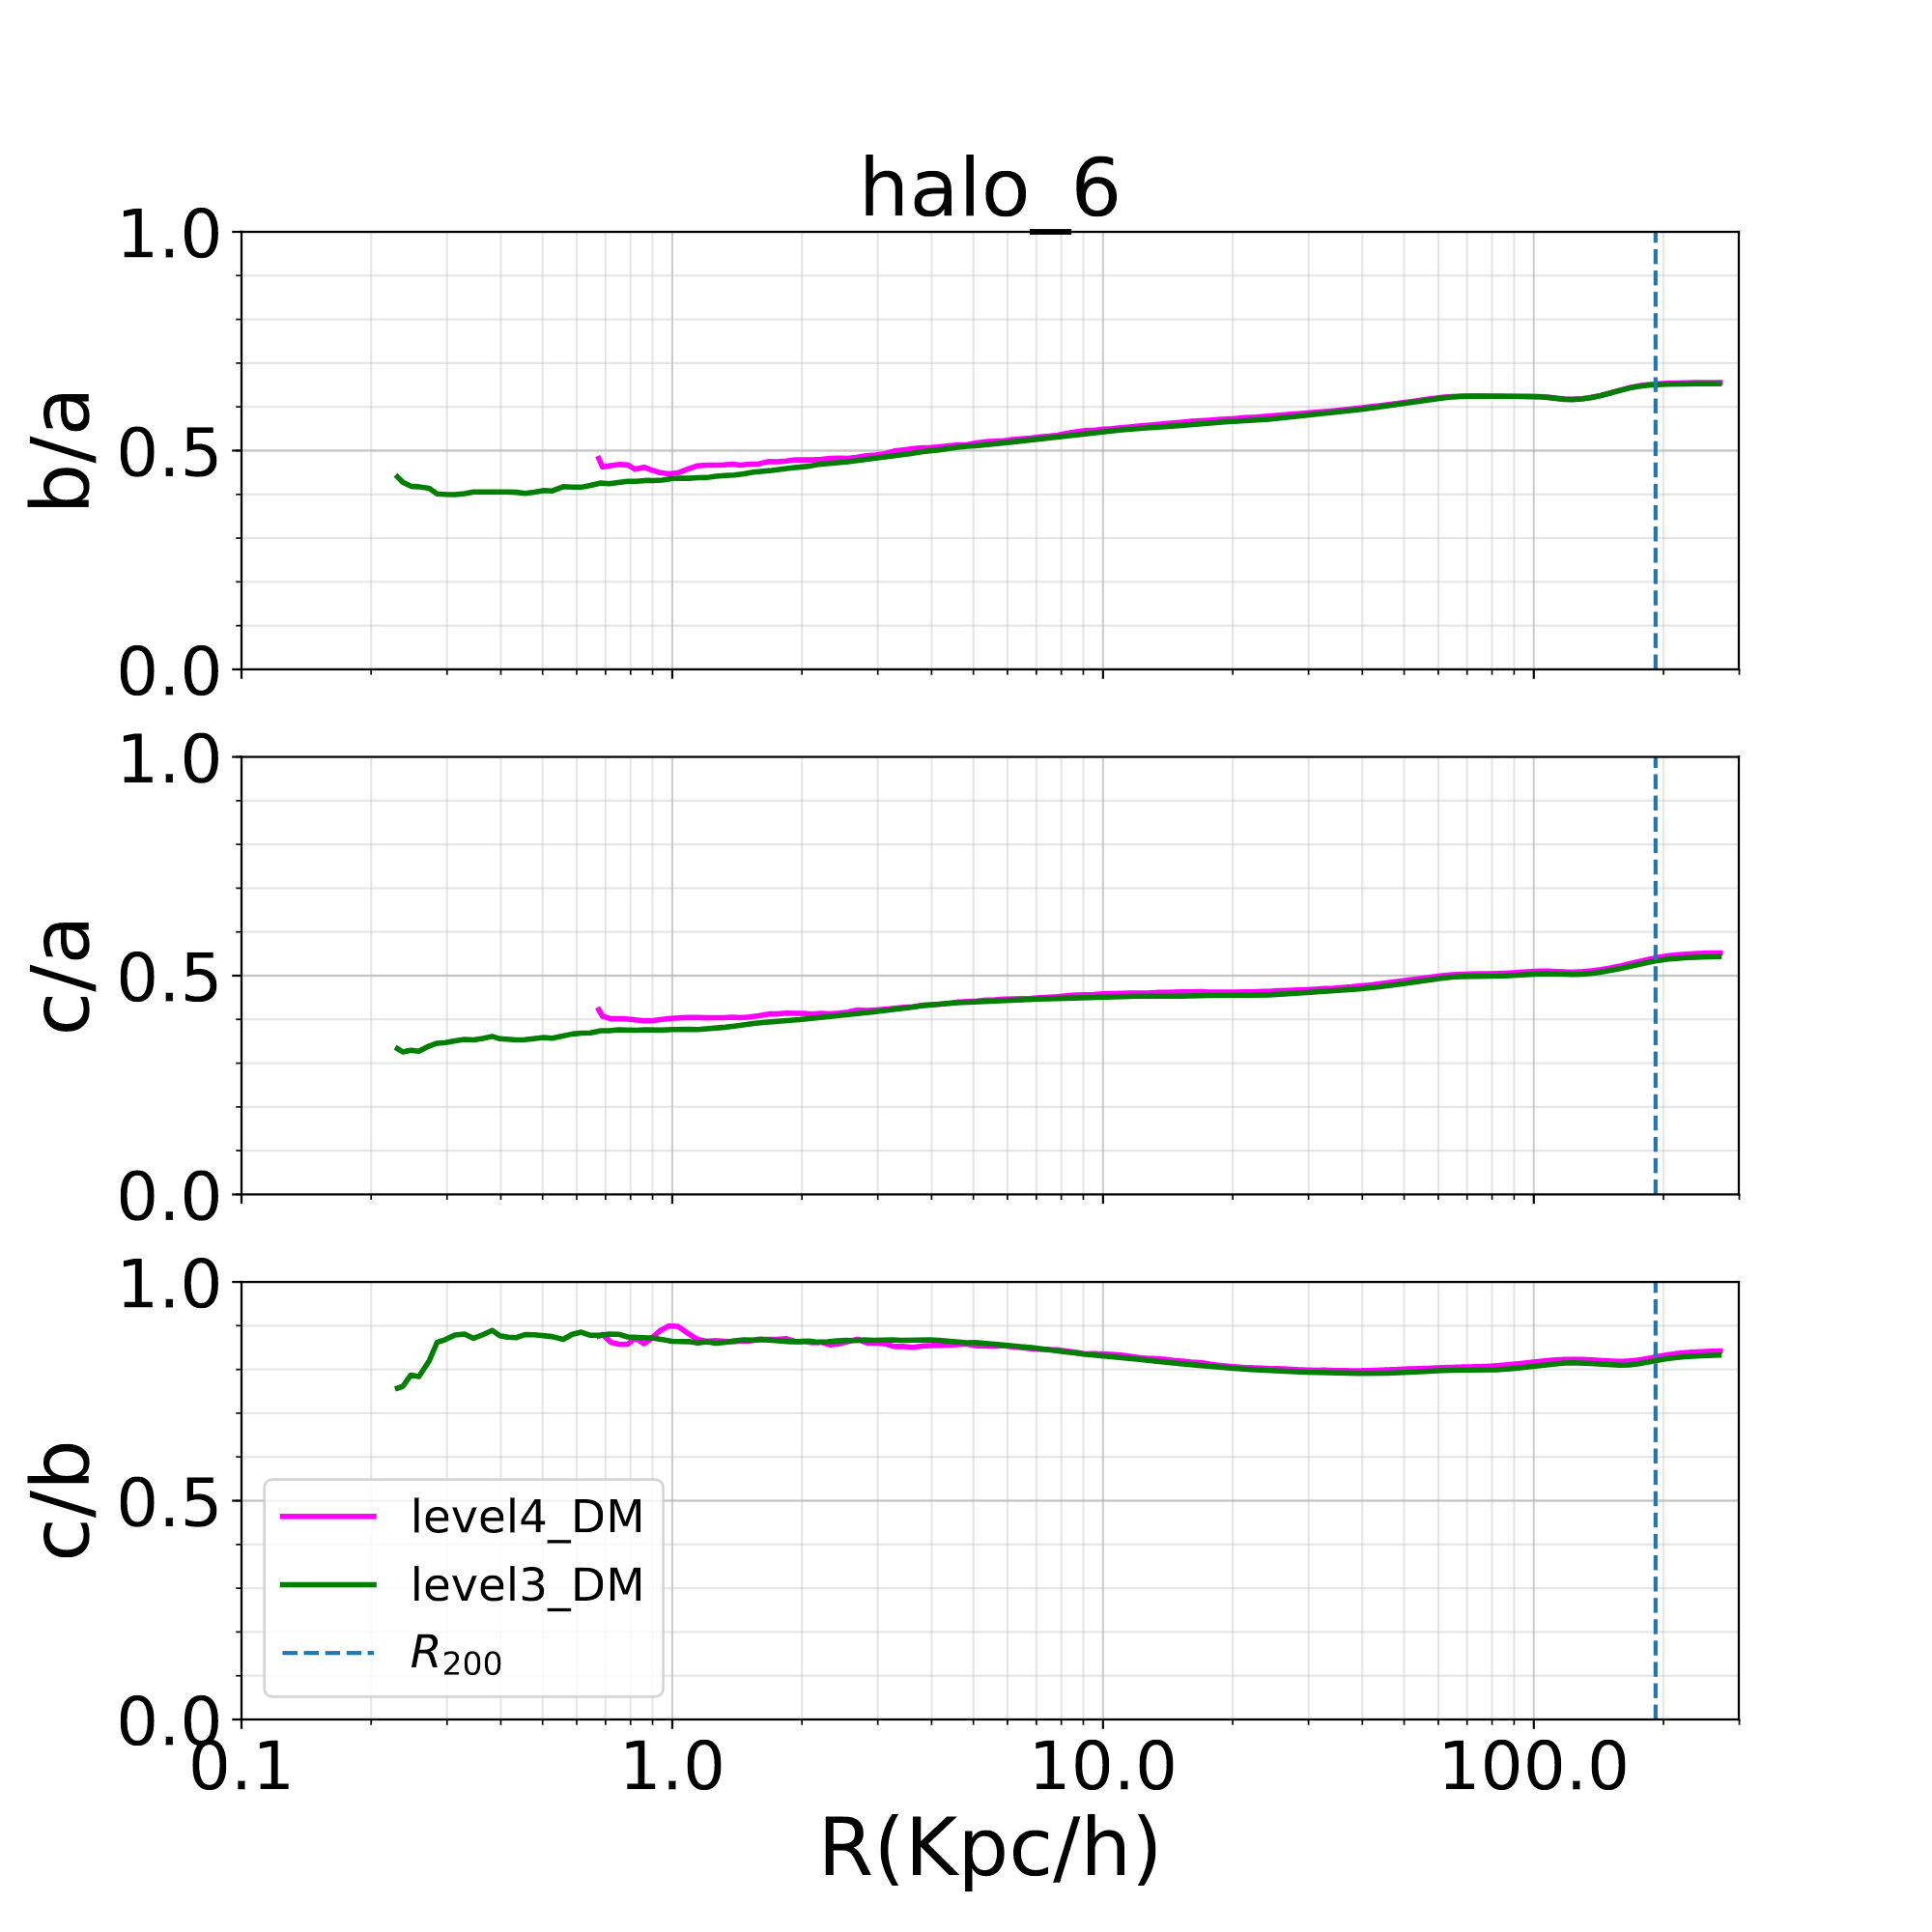
\includegraphics[width=0.5\columnwidth]{./pics/Convergence/halo6_DM_3Vs4_good.png}}
  \hfill
  \subfloat[halo 27 MHD]{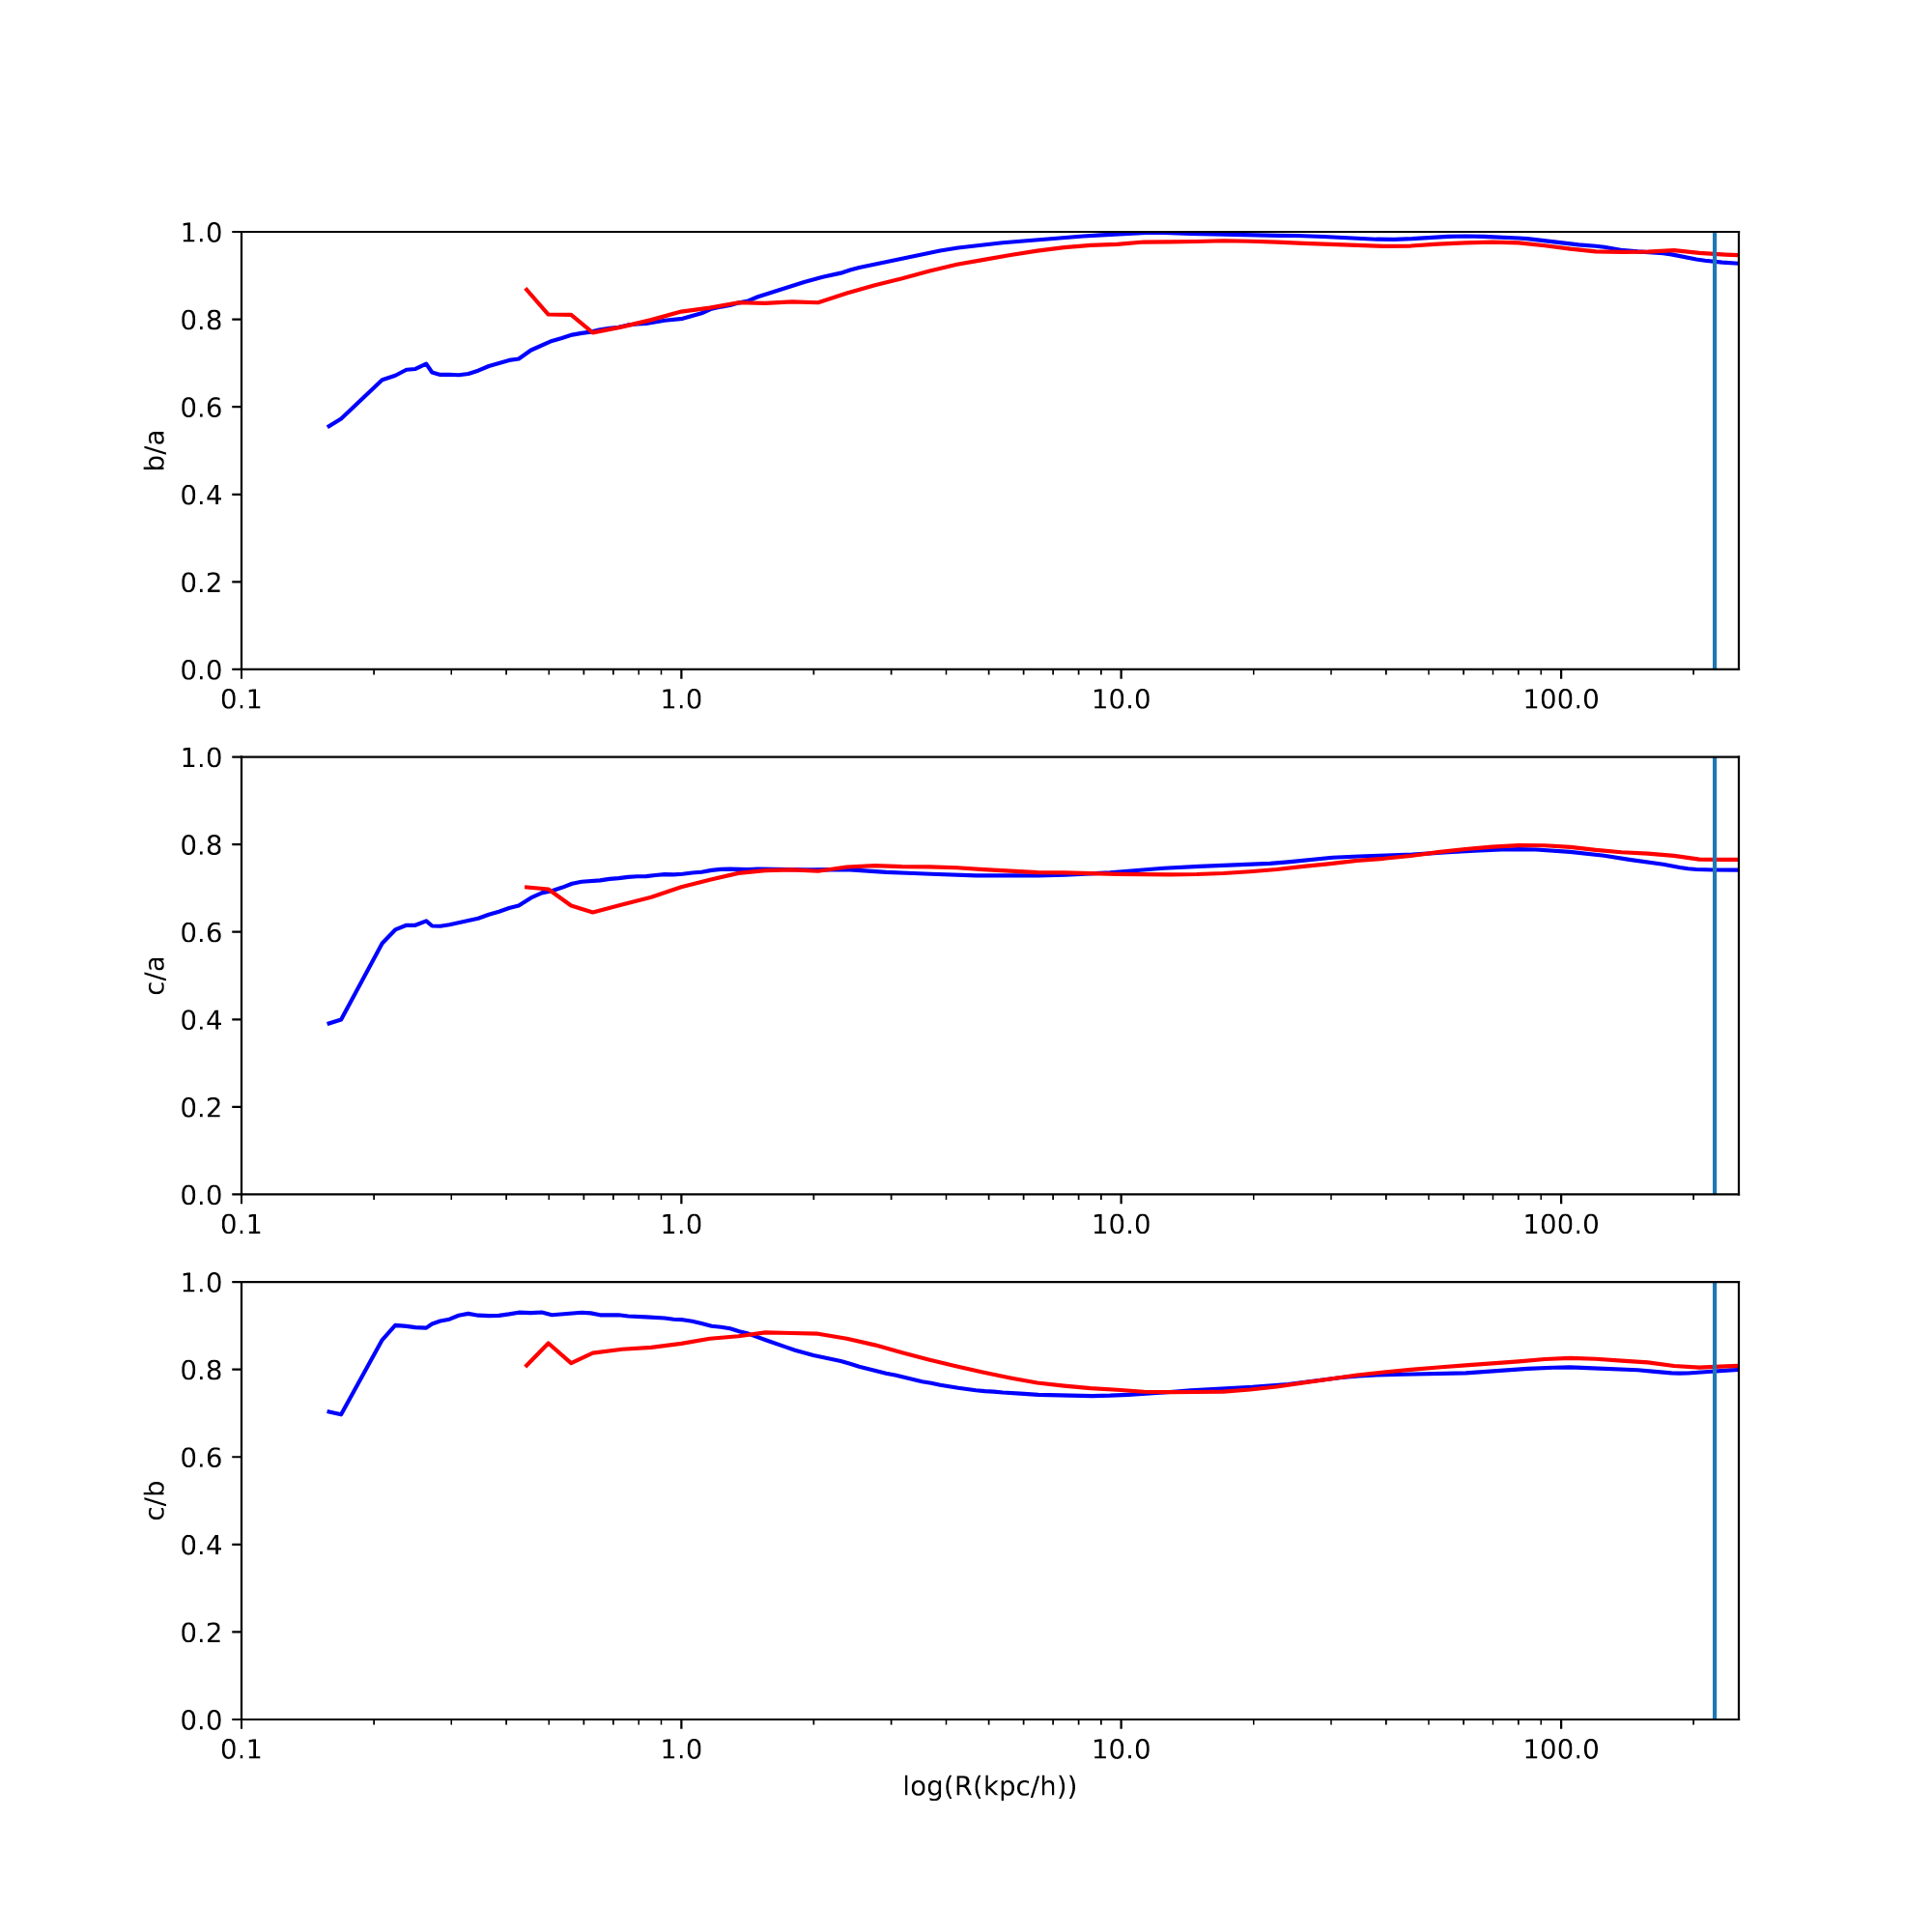
\includegraphics[width=0.5\columnwidth]{./pics/Convergence/halo27_MHD_3Vs4_good.png}}
  \caption{Level 3 (green) \& 4 (pink) radial profiles of axial ratios for halo 6 (DM) \& 21 (MHD). Here, it is clear that there is good agreement on the calculated quantities for both levels of resolution.}
  \label{fig:goodConvergence}
\end{figure}



\begin{figure}[!ht]
  \centering
  \subfloat[halo 16 DM]{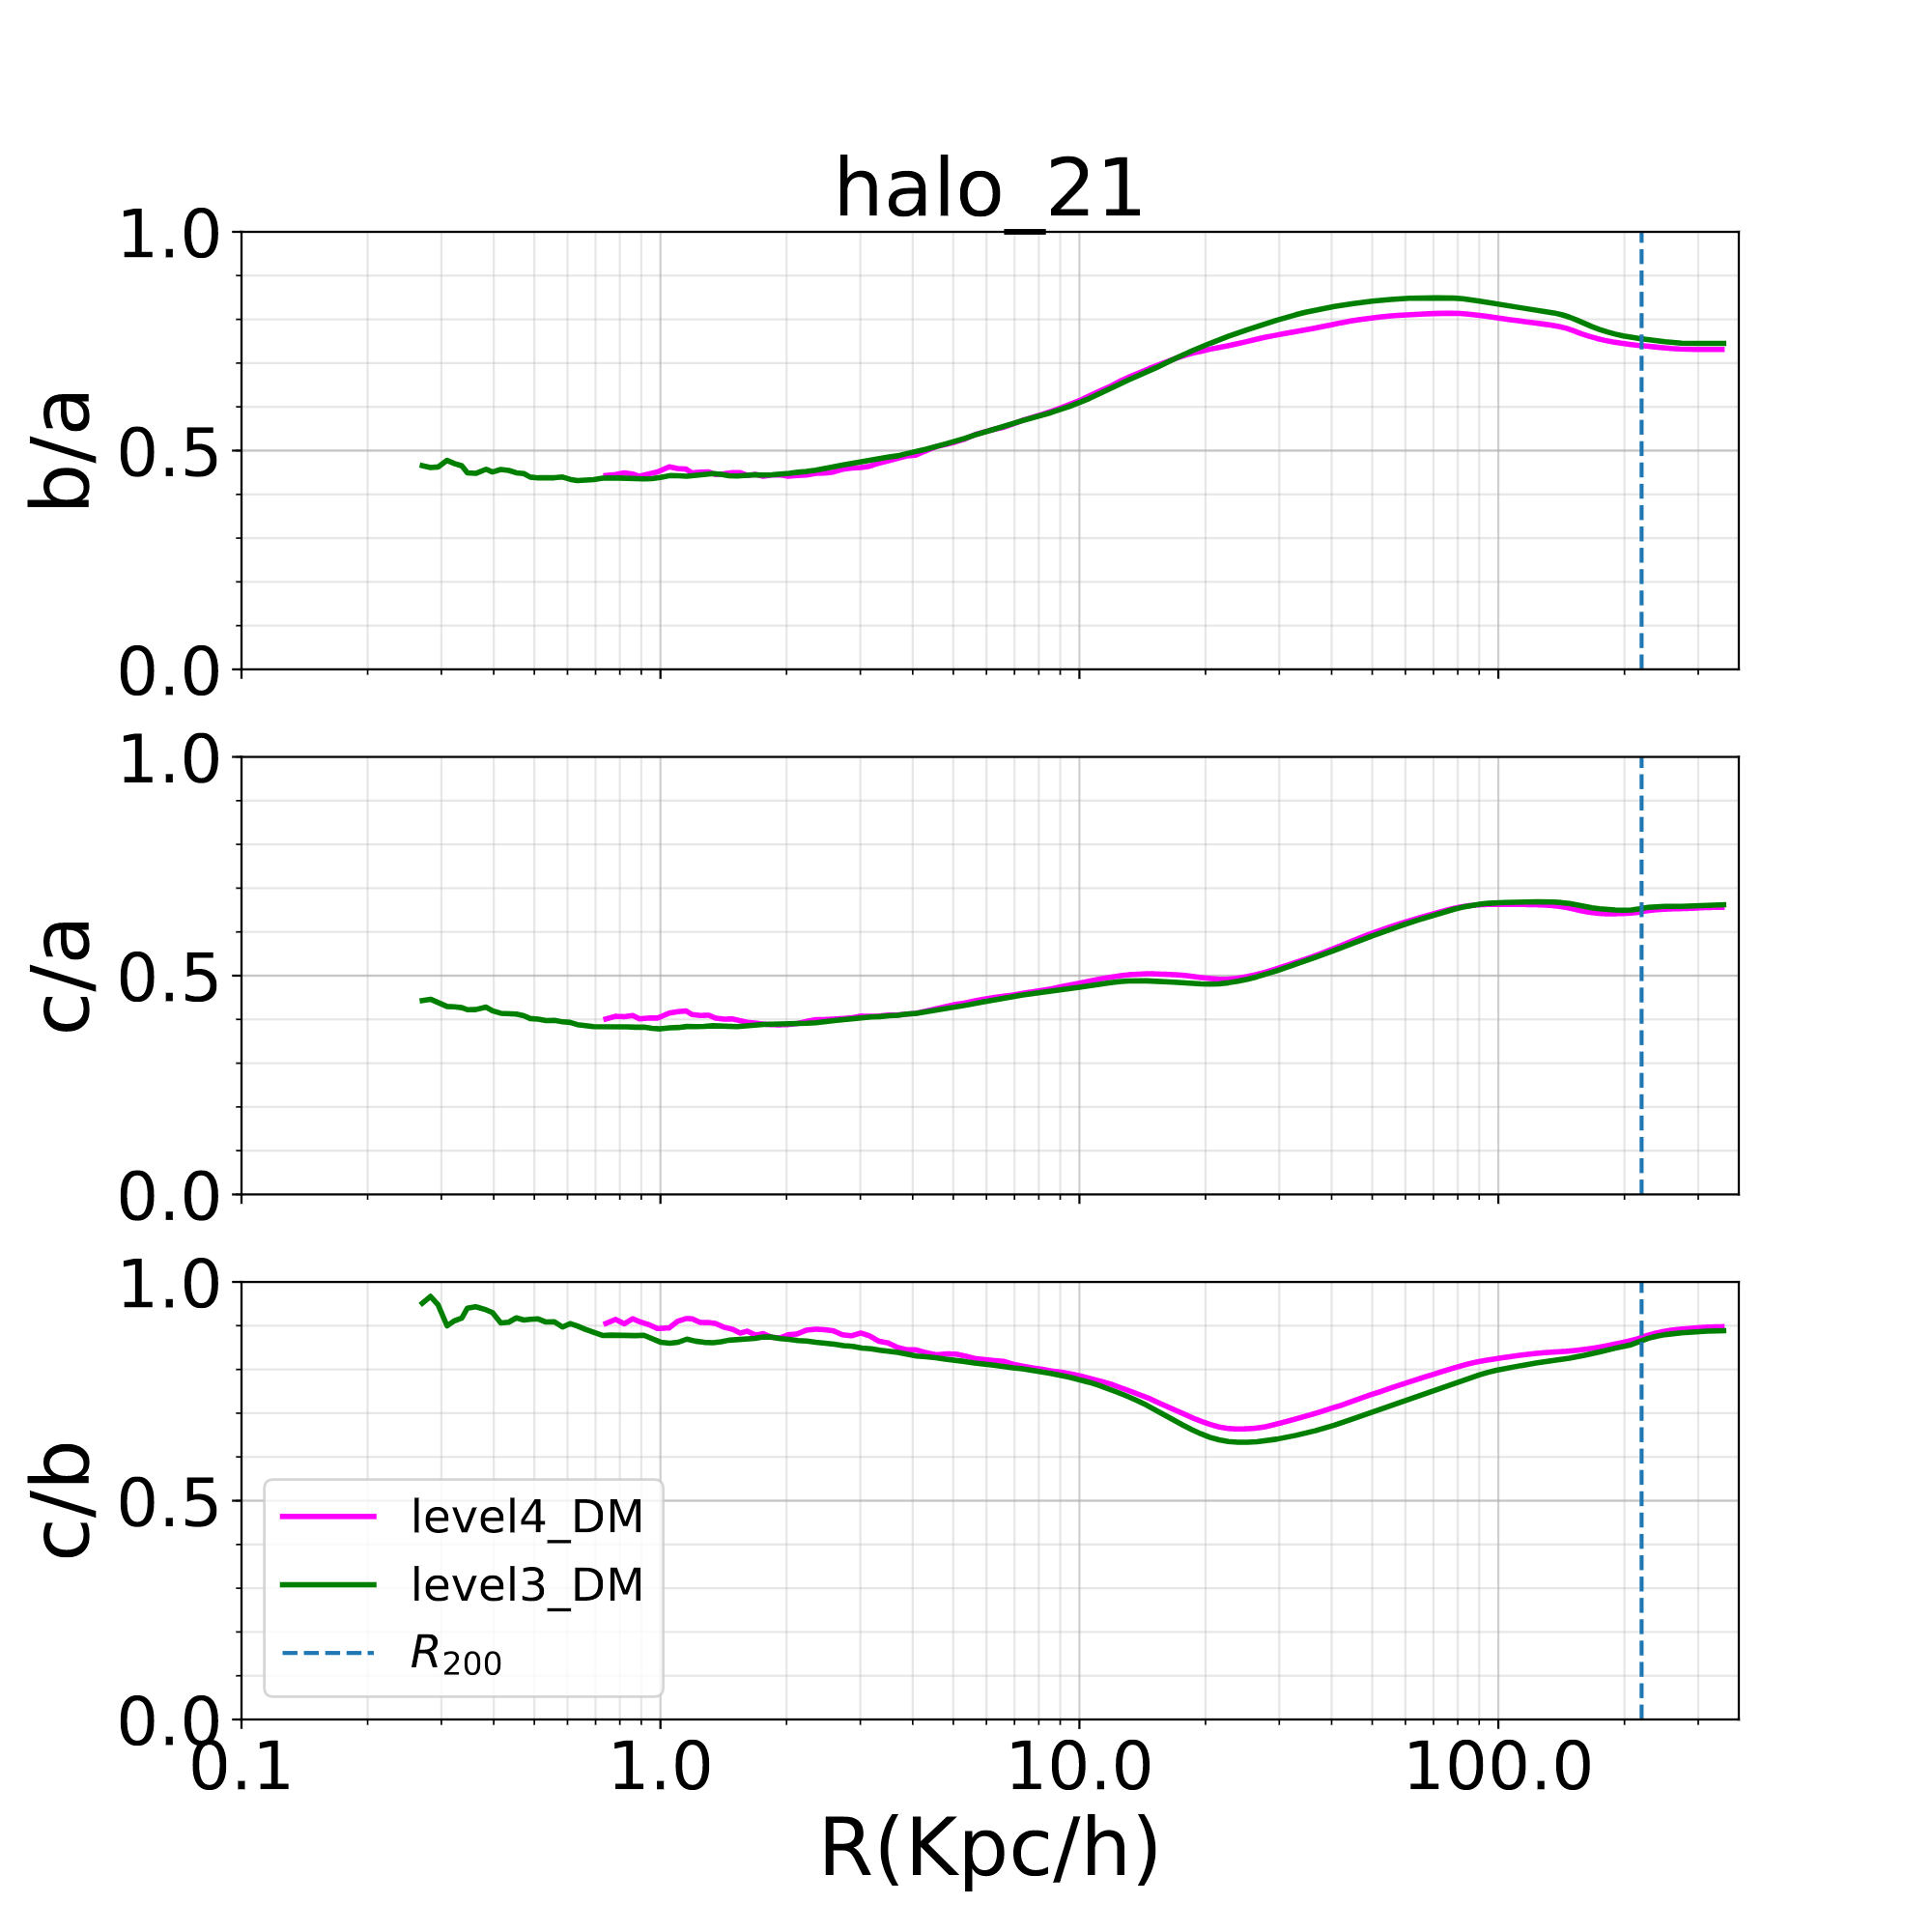
\includegraphics[width=0.5\textwidth]{./pics/Convergence/halo21_DM_3Vs4_bad.png}}
  \hfill%\hspace{-0.5em}
  \subfloat[halo 23 MHD]{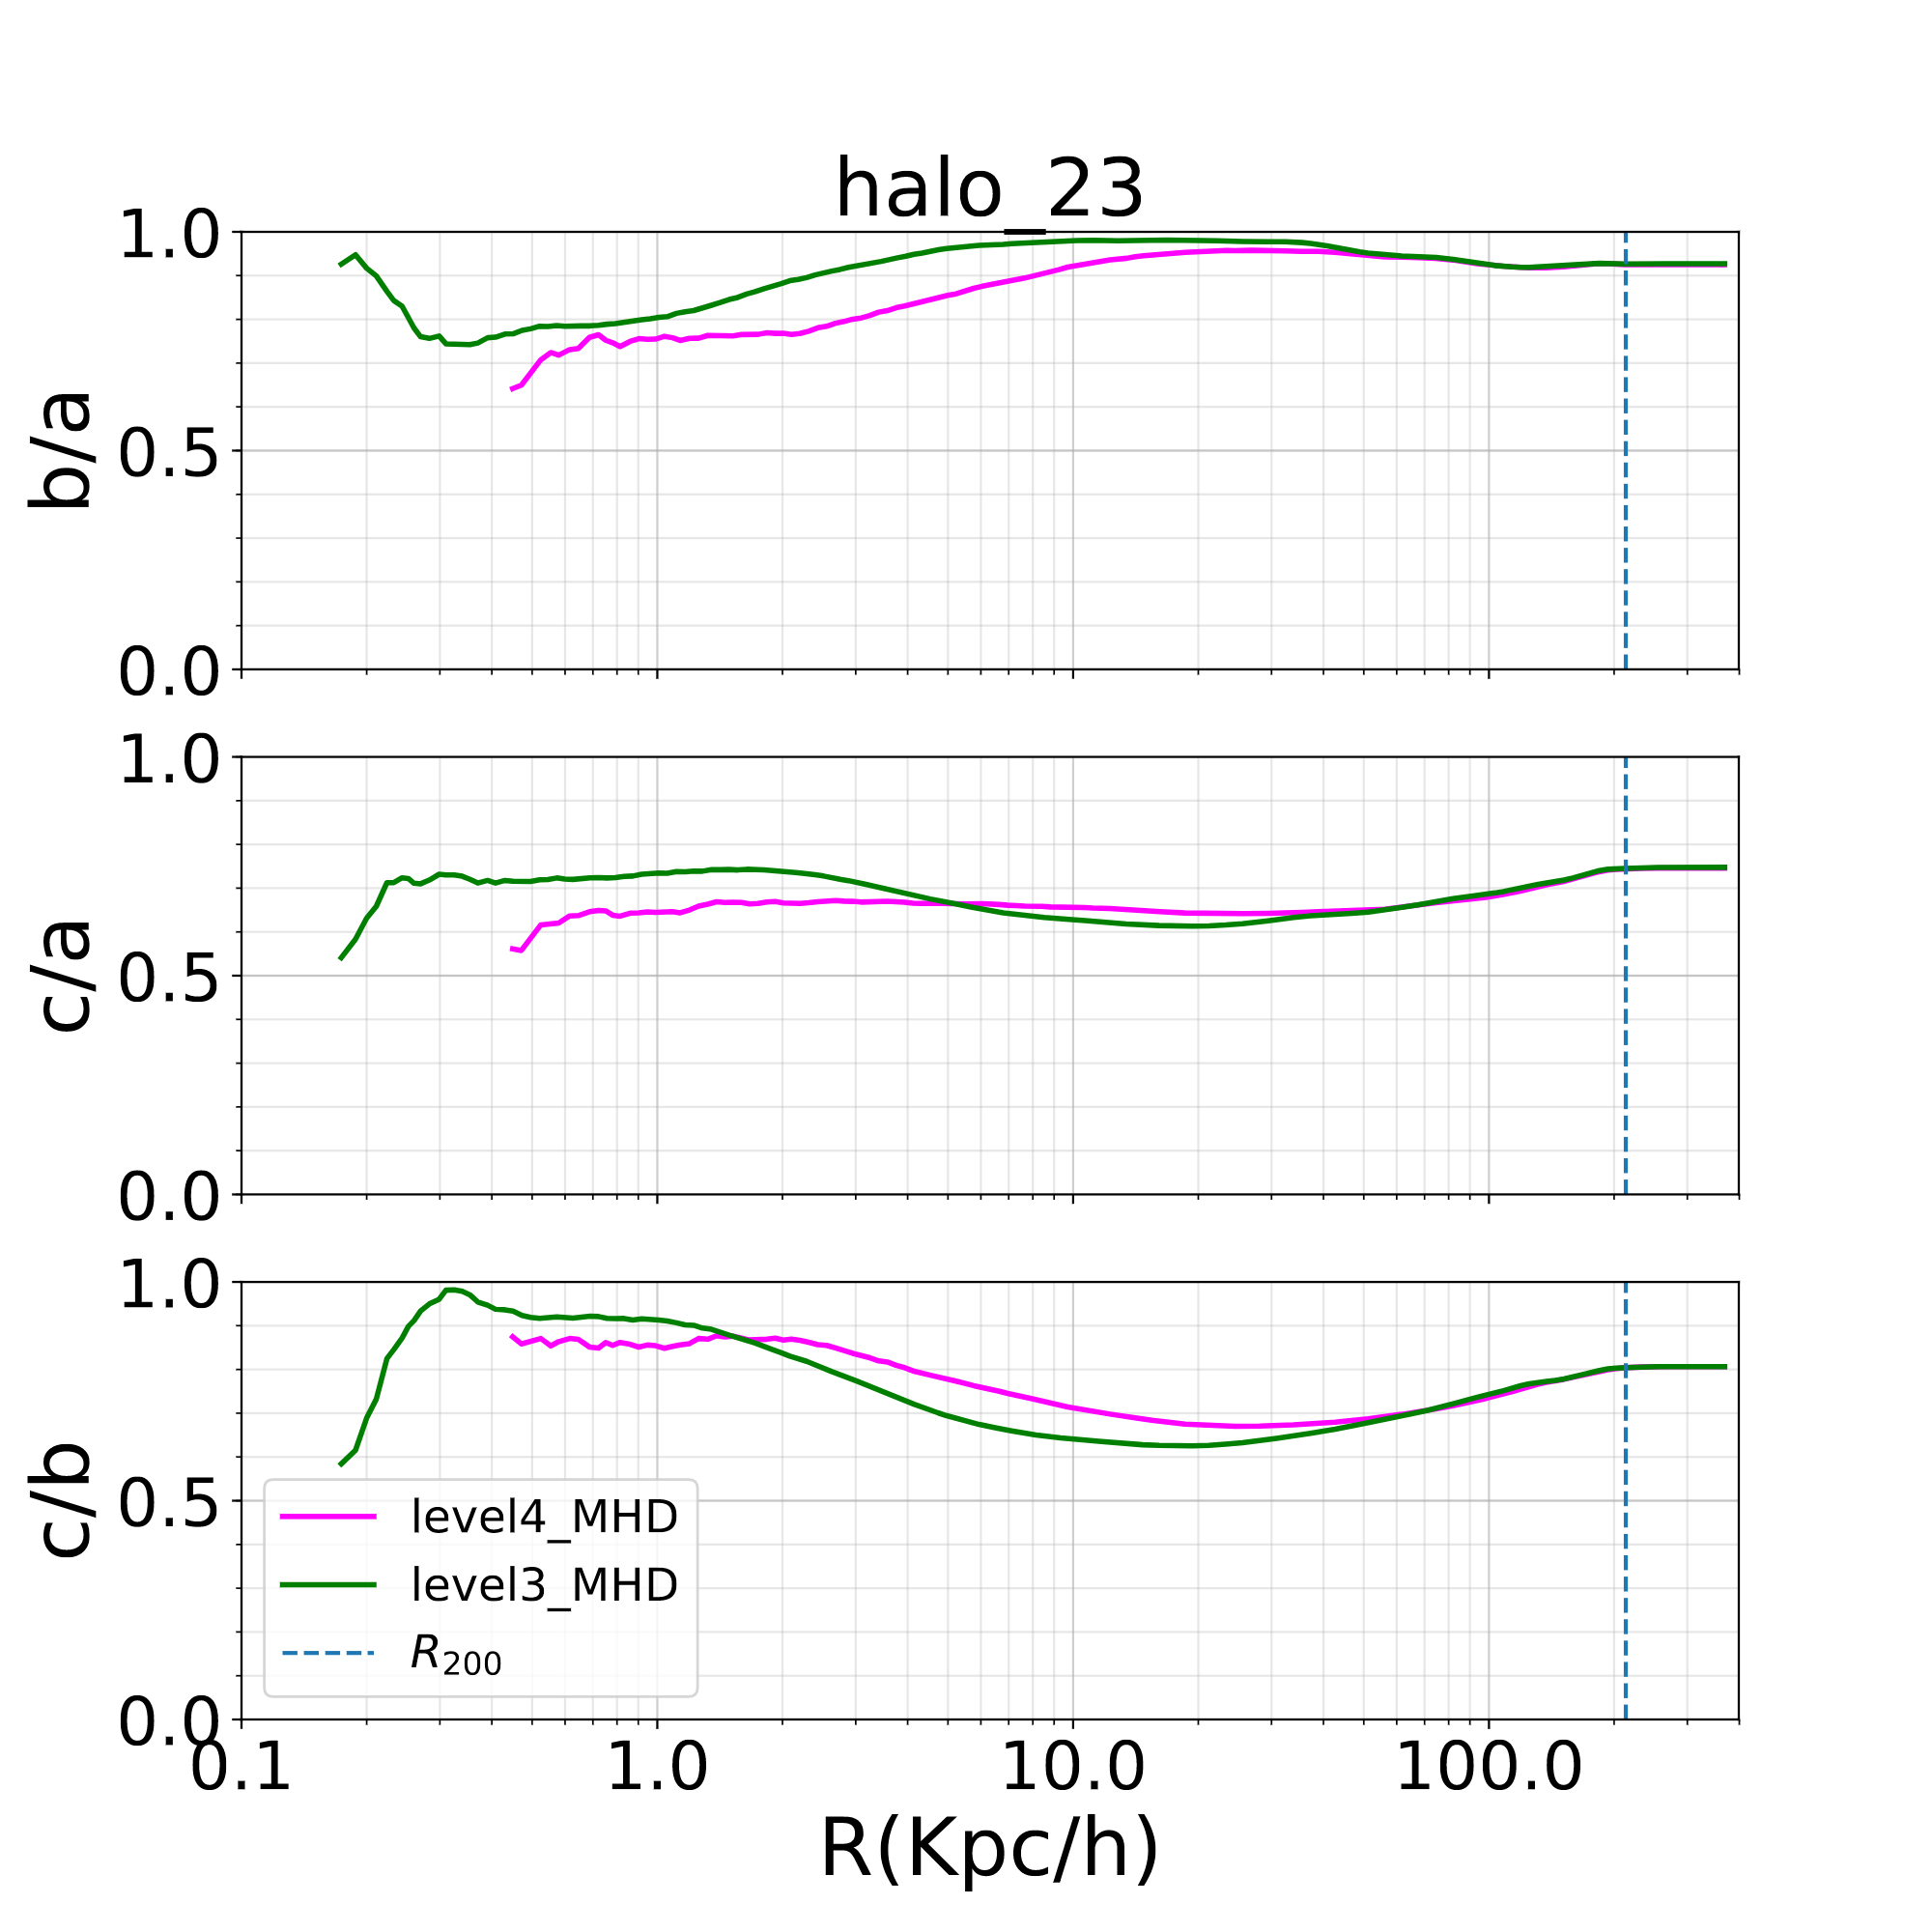
\includegraphics[width=0.5\textwidth]{./pics/Convergence/halo23_MHD_3Vs4_bad.png}}
  \caption{Level 3 (green) \& 4 (pink) radial profiles of axial ratios for halo 16 (DM) \& 23 (MHD). Here, axial ratios show slow convergence. }
  \label{fig:badConvergence}
\end{figure}


For instance, by simple inspection, we notice that there is no apparent systematic way in which resolution affects the halo shape. That is, at some radii the highly-resolved level 3 halo appears rounder and at other radii it seems more triaxial. This is important for our study as we focus on the analysis of the triaxial properties of the halo. Incidentally, DM-only halos remain unchanged with the exemption of the radial regimes where the number of particles affects our shape-calculating method. However, for MHD simulations, the resolution of baryons has a global influence over the axial ratios. We suspect this is caused by continuous exposition of particles due to the resolution-sensible baryonic potential. Nevertheless, further calculations are needed to confirm the cause of these discrepancies.\\

Consequently, to rule out our shape method as a cause of these resolution differences, we decide to isolate the few-particle effect on our calculations. To do this, we randomly select DM particles from level 3 halos at $z=0$ to produce 10 samples of approximately the same size as level 4 simulations. We then calculate this few-particle effect, which we show in figures \ref{fig:convergence}. For each radius, we compute the mean and standard deviation of the set of 10 randomly sampled shapes and illustrate a 3-sigma range around the mean curve to compare with the respective level 4 shape values.\\  

From graphics on \ref{fig:convergence}, it is clear that the fractional difference is not actually significant and remains under $1\%$ for the majority of the radial profile. It becomes important for radii less than 1Kpc due to the lack of particles for approximating an elliptical shape. This is corroborated by the $3\sigma$ range, which also becomes evident around 1Kpc. We deduce from this analysis that for radii bigger than 1Kpc, the differences of level 3 and level 4 ellipses cannot be explained as an effect of the lack of particles affecting our shape method. This is a confirmation that all kinds of matter are directly affected by resolution due to precision-sensitive events on the history of formation or because the numerical gravitational potential of matter continuously influences surrounding structures. Either way, even for the most resolution-biased cases, we can say that, for the purposes of this study, convergence is achieved to a reasonable extent for $r>$10Kpc and that we must be careful when interpreting axial ratios at $r<$5Kpc. \\  

\begin{figure}[!ht]
  \centering
  \subfloat[halo 24 MHD]{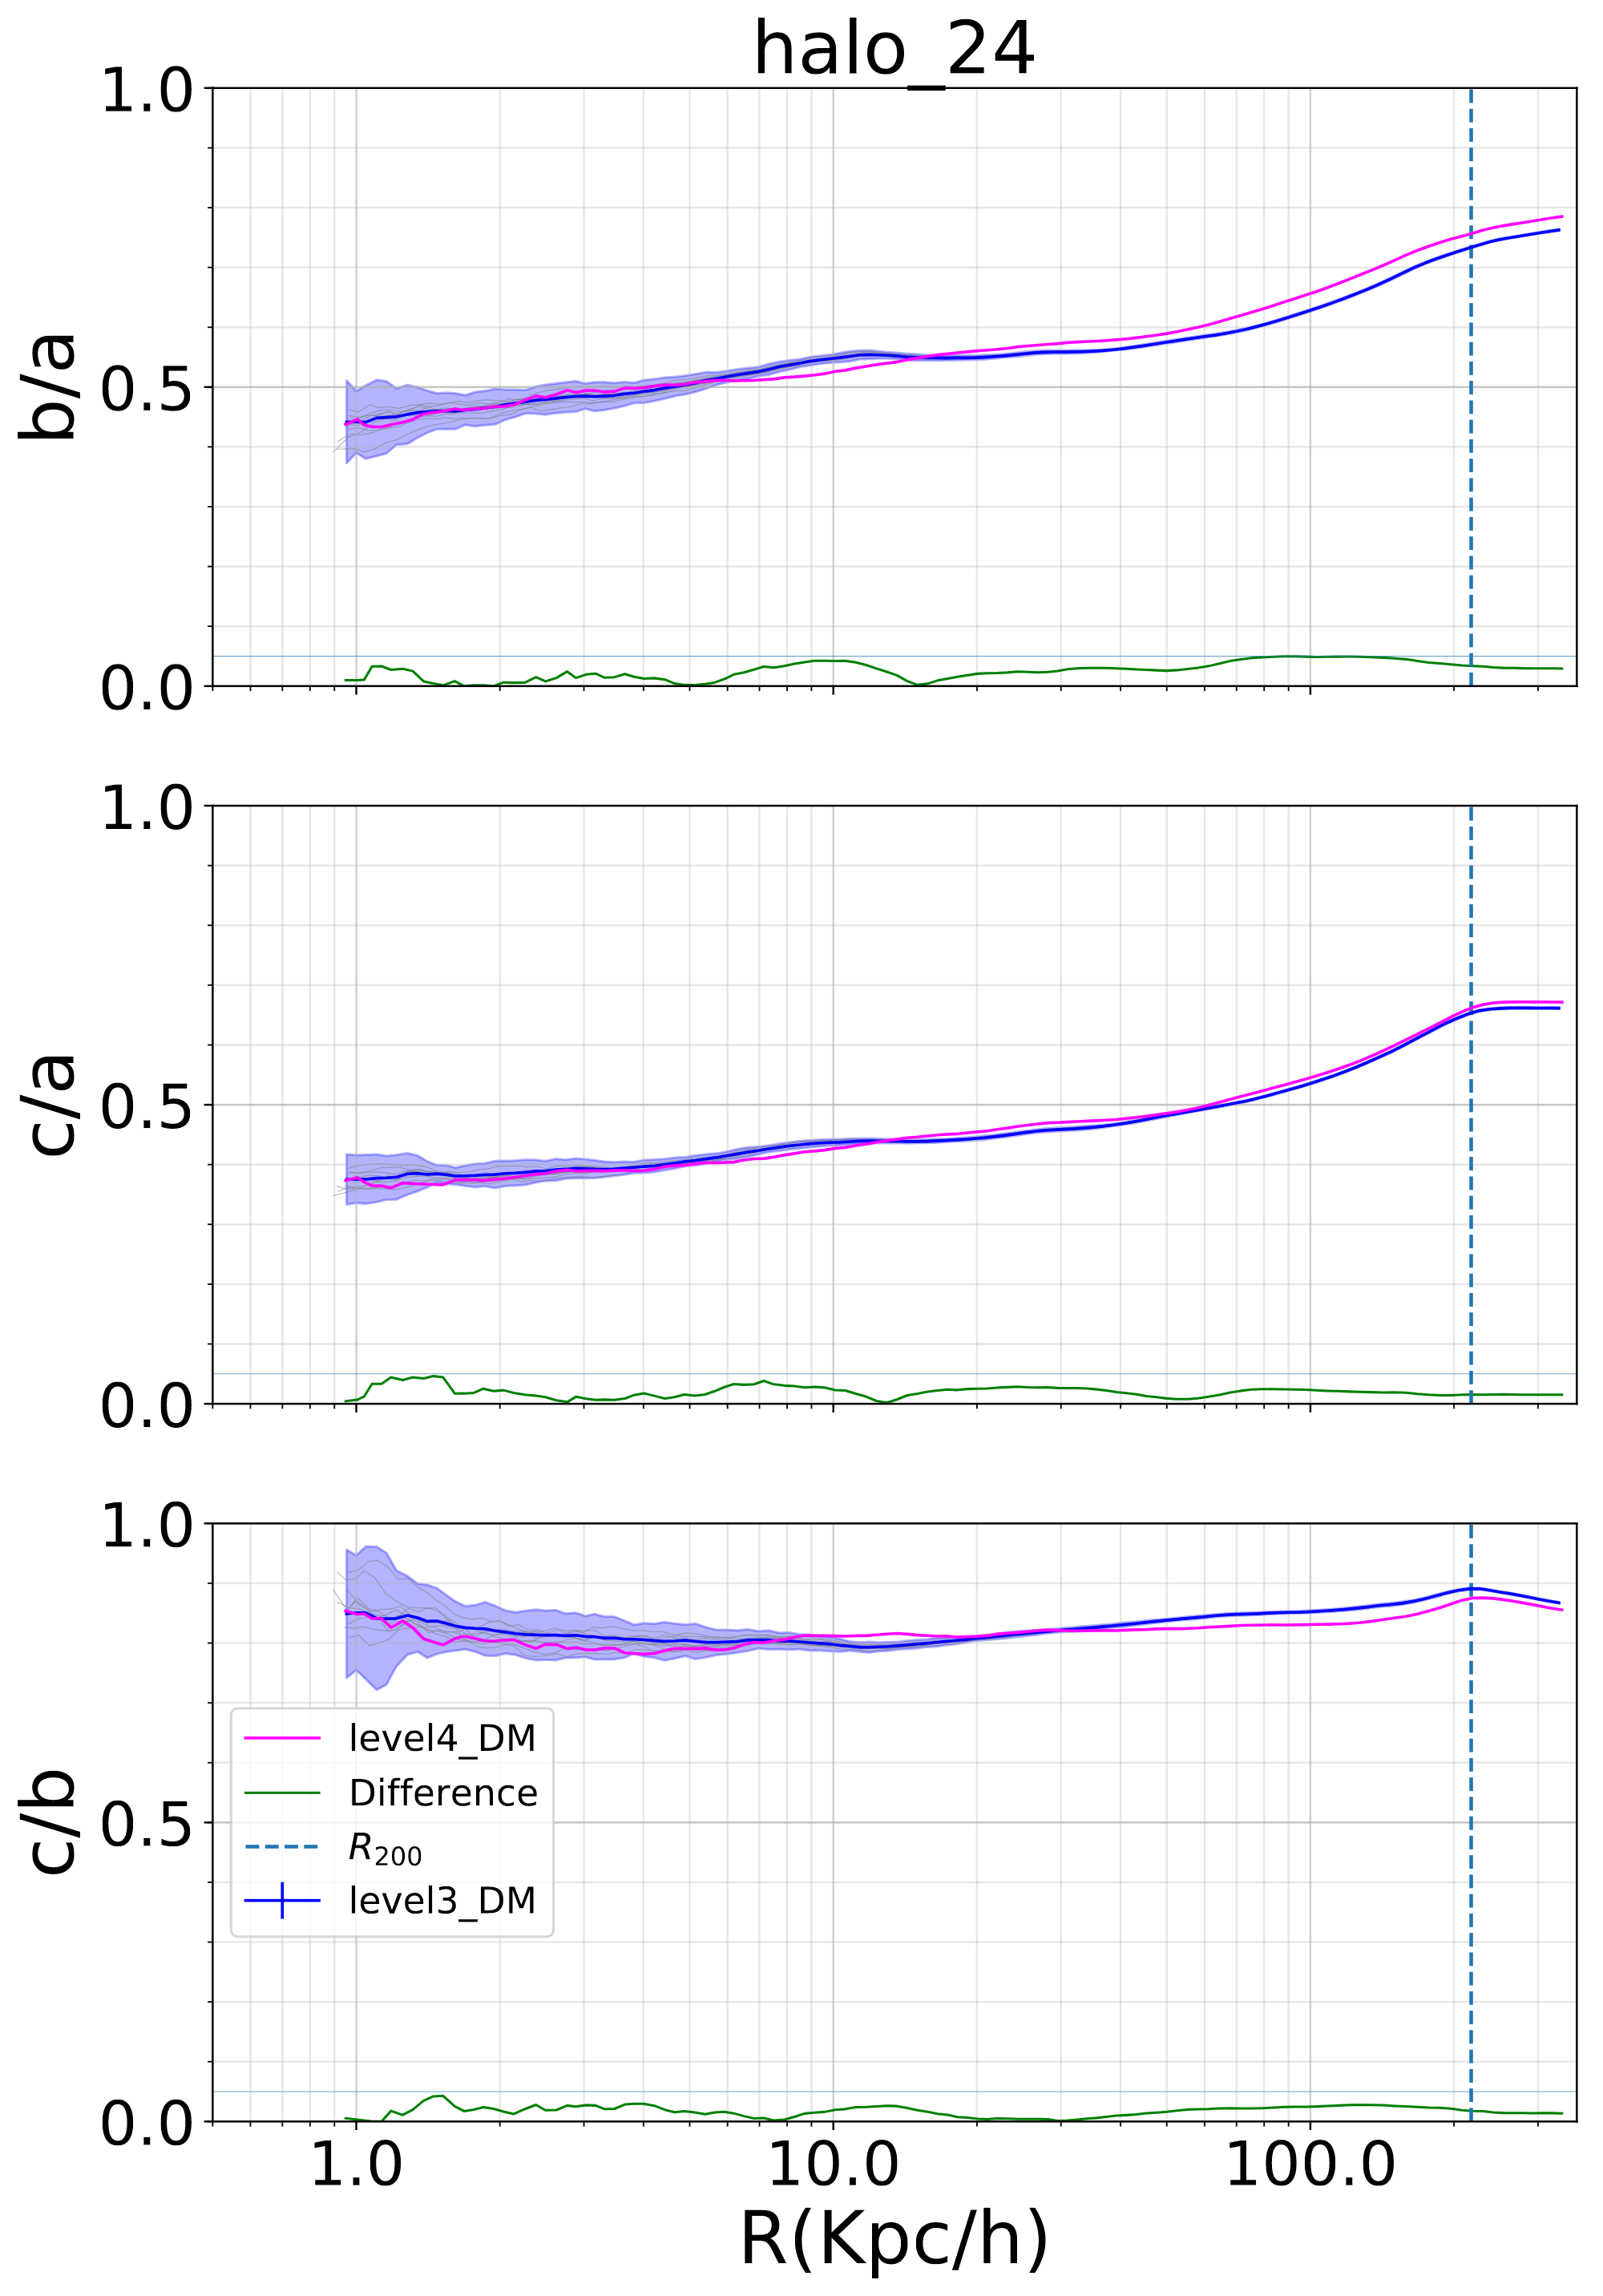
\includegraphics[width=0.5\columnwidth]{./pics/Convergence/rand_conv_halo24_DM.png}}
  \hfill
  \subfloat[halo 24 DM]{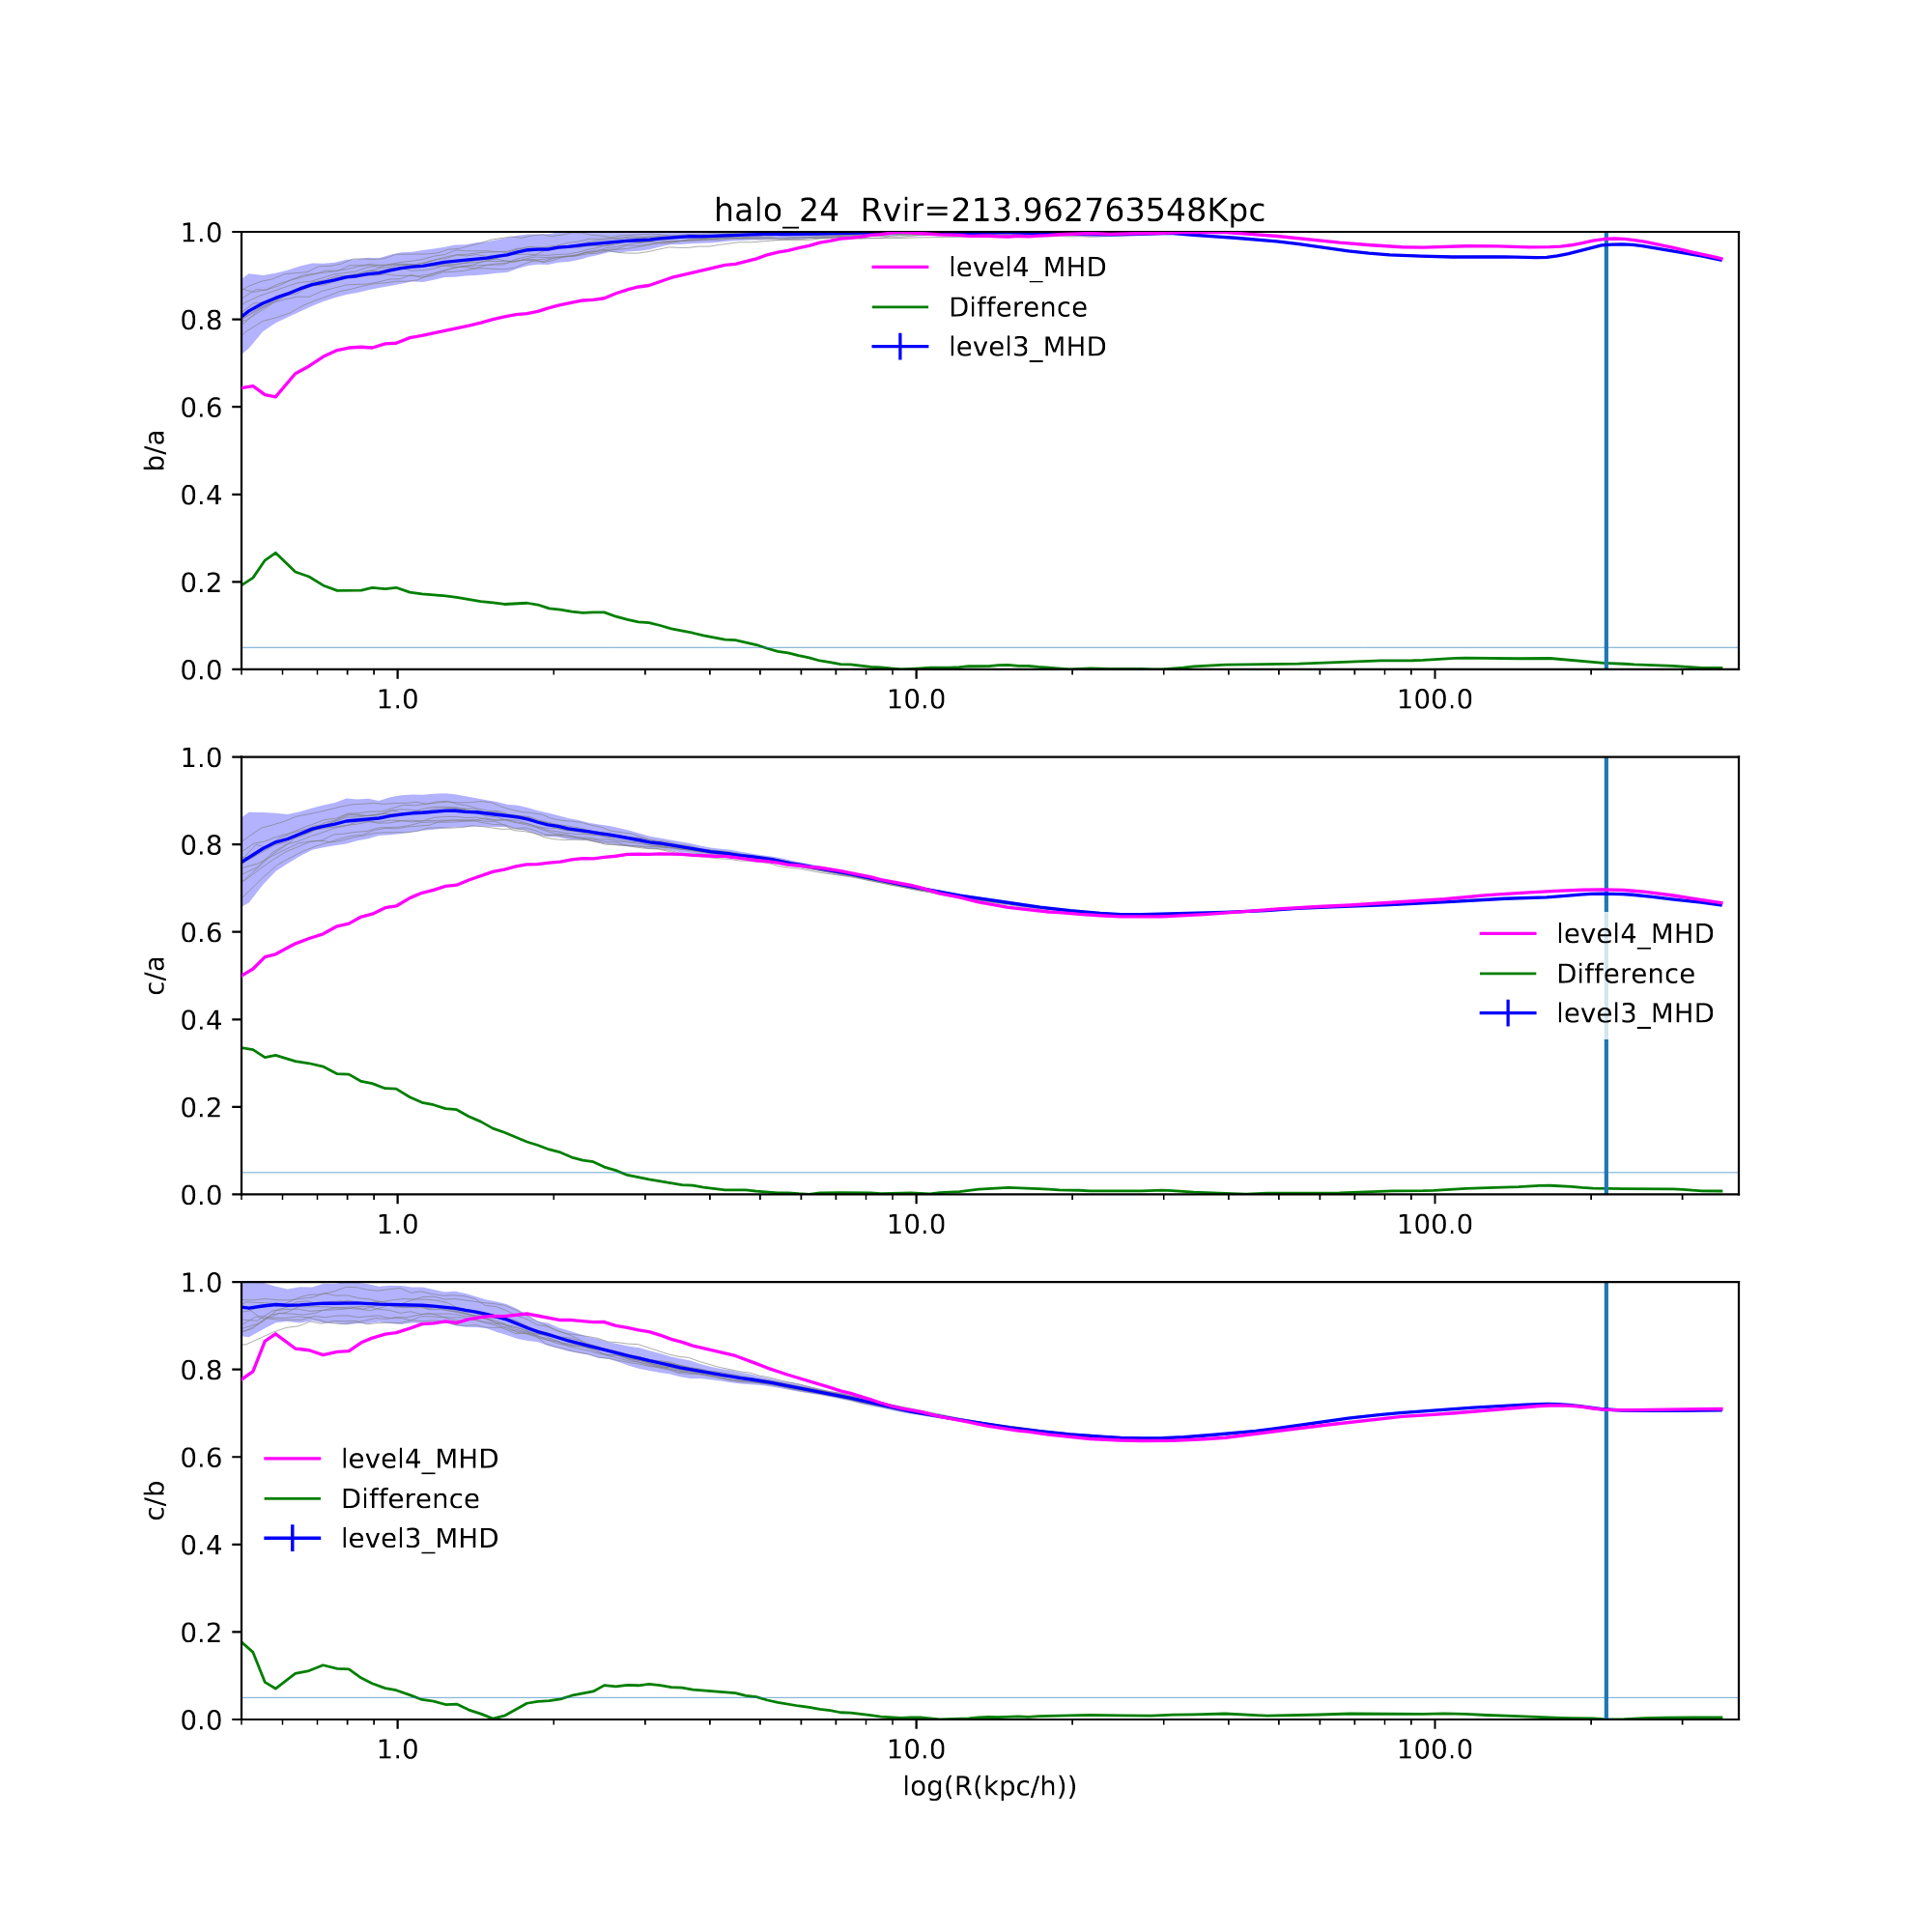
\includegraphics[width=0.5\columnwidth]{./pics/Convergence/rand_conv_halo24_MHD.png}}
  \caption{The few-particle effect on the axial ratios convergence for halo 24 (DM \& MHD). Here level4 curves (magenta) are compared to  the 3$\sigma$ range (clear blue) of the random-sampled curves from level3 (solid blue). We deduce from the fractional difference (green) that discrepancies at $r>>1$Kpc cannot be explained solely with the few-particle bias. }
  \label{fig:convergence}  
\end{figure}

\section{The radial dependence of axial ratios}
One of our first results regarding the halo shape is related to its evolution in terms of the radius. As stated earlier, we expect from previous work that the shape does not remain constant along the radius \cite{Vera-Ciro_et_al._2011}. Specifically, after some time, halos are gradually constructed from inner shells to outer shells through constant accretion of matter from cosmic structures \cite{Tormen_et_al._1997,Tormen_et_al._1998}. Inner shells tend to conserve their shape as a consequence of being shielded from the outside by Gauss law. Outer shells, on the other side, are continuously affected by the gravitational potential from the inside, which makes them prone to the scattering of particles, which randomizes their orbital parameters. Therefore, this inner gravitational potential has a \textit{rounding} effect on the outskirts. For this reason, we expect that halos are more triaxial on inner regions and more spherical at bigger radii. This effect has been corroborated on multiple cosmological simulations of different degrees of realism \cite{Frenk_et_al._1988,Dubinski_and_Carlberg_1991,Warren_et_al._1992,Cole_and_Lacey_1996,Hayashi_et_al._2007,Bett_et_al._2007,Vera-Ciro_et_al._2011}. \\


\begin{figure}[!ht]
  \centering
  \subfloat[halo 27 DM shape at small radius]{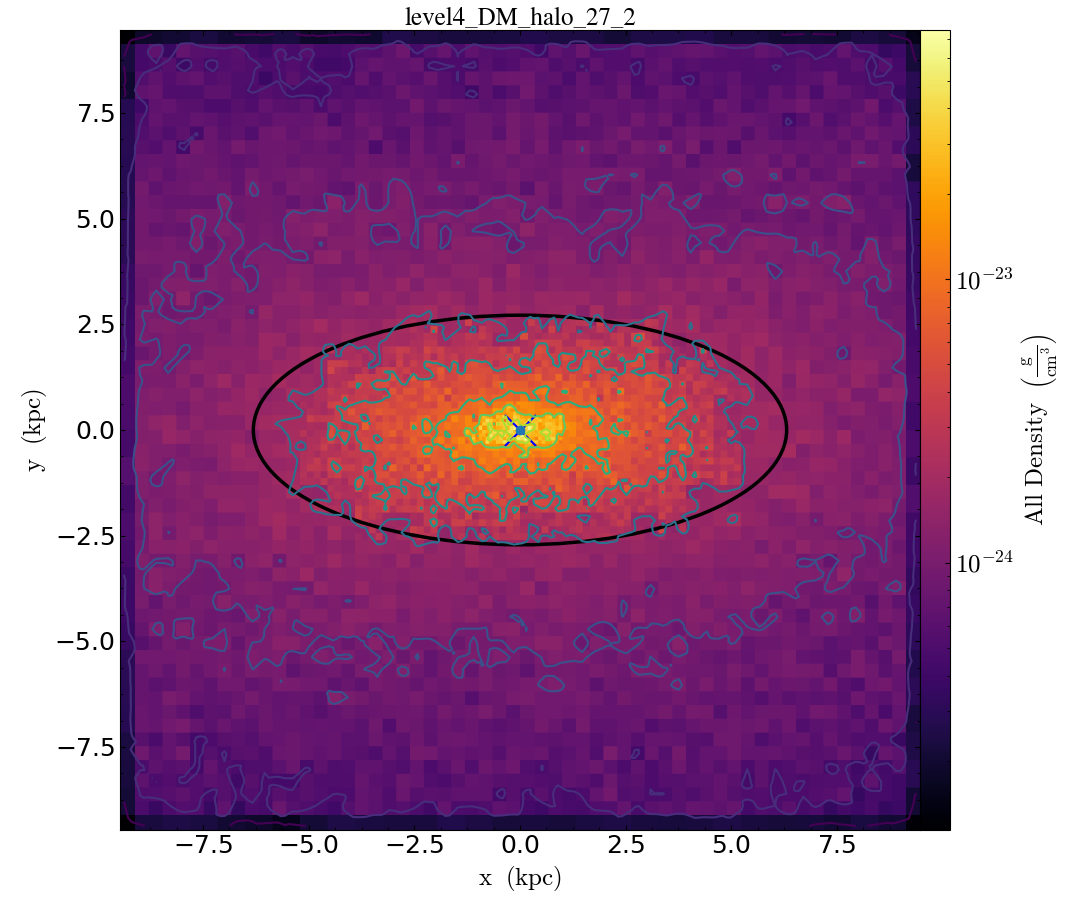
\includegraphics[width=0.5\columnwidth]{./pics/MHD_Vs_DM/level4_DM_halo_27_inner.png}}
  \hfill
  \subfloat[halo 27 DM shape at big radius]{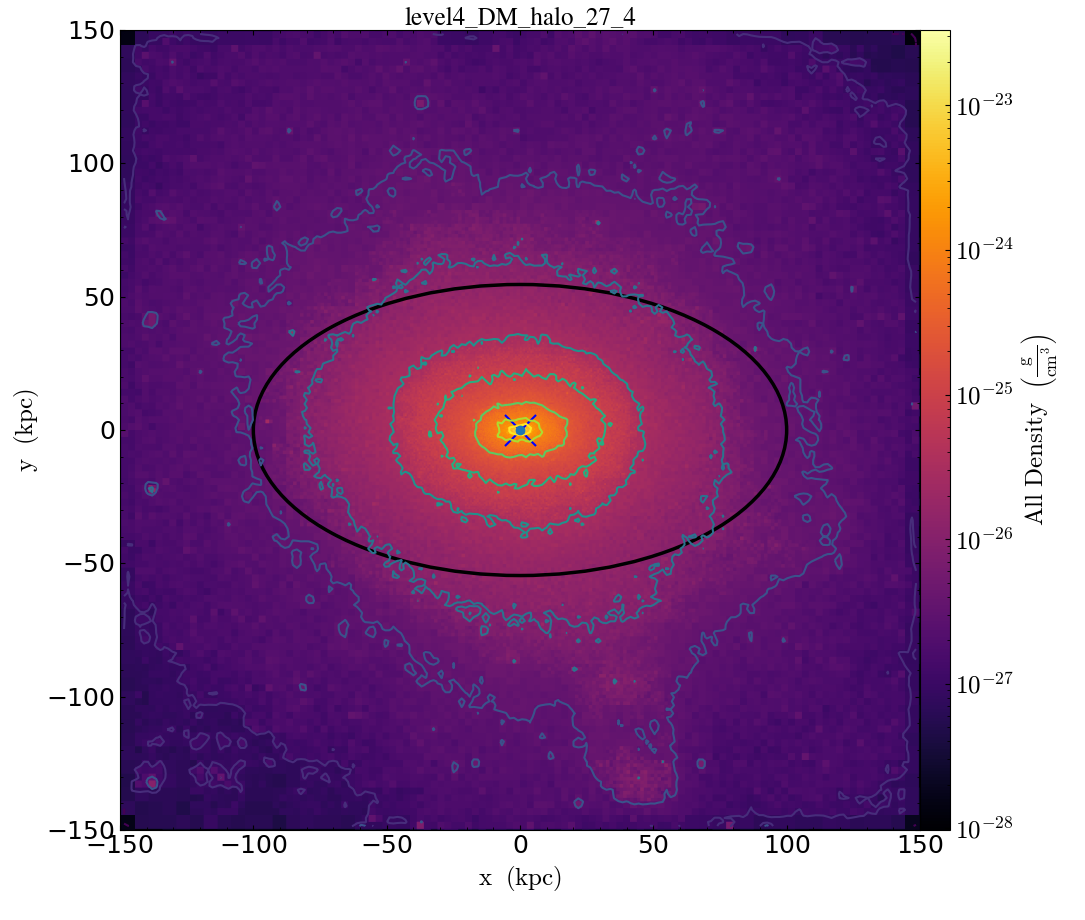
\includegraphics[width=0.5\columnwidth]{./pics/MHD_Vs_DM/level4_DM_halo_27_outter.png}}
  \hfill
  \subfloat[halo 27 MHD shape at small radius]{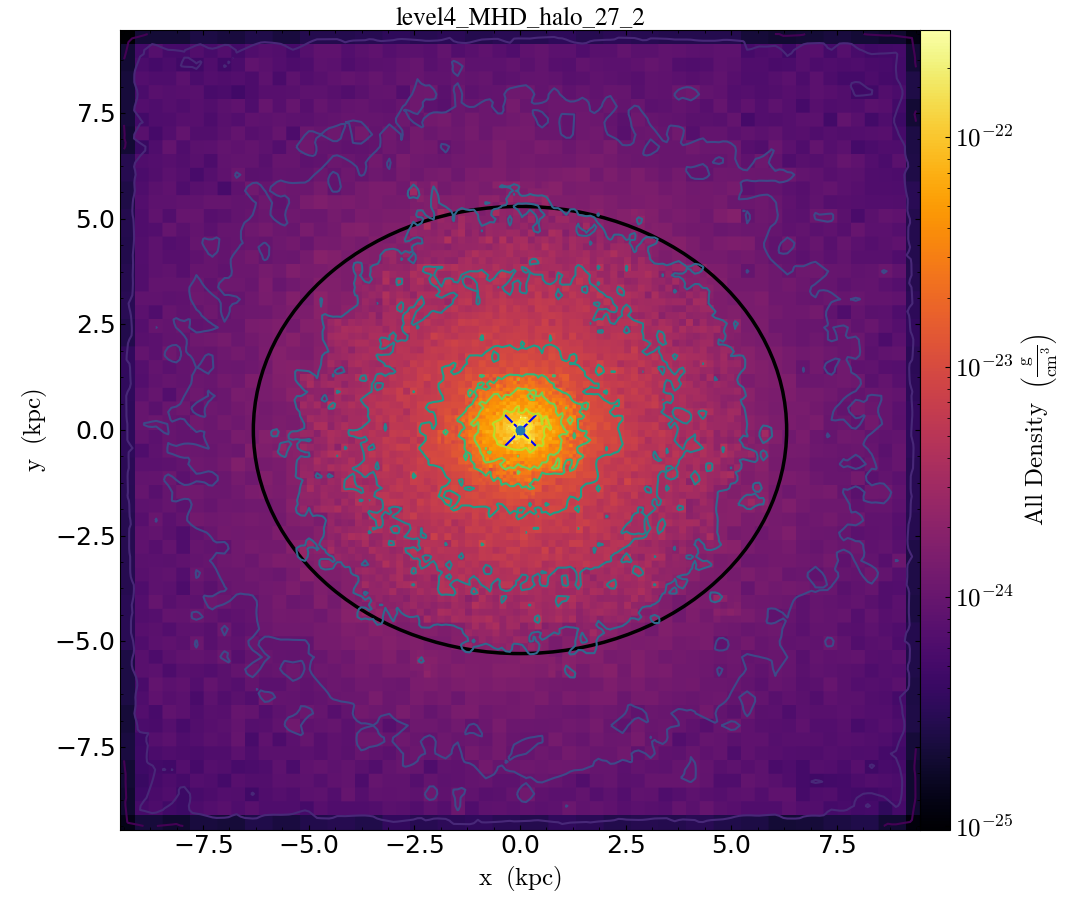
\includegraphics[width=0.5\columnwidth]{./pics/MHD_Vs_DM/level4_MHD_halo_27_inner.png}}
  \hfill
  \subfloat[halo 27 MHD shape at big radius]{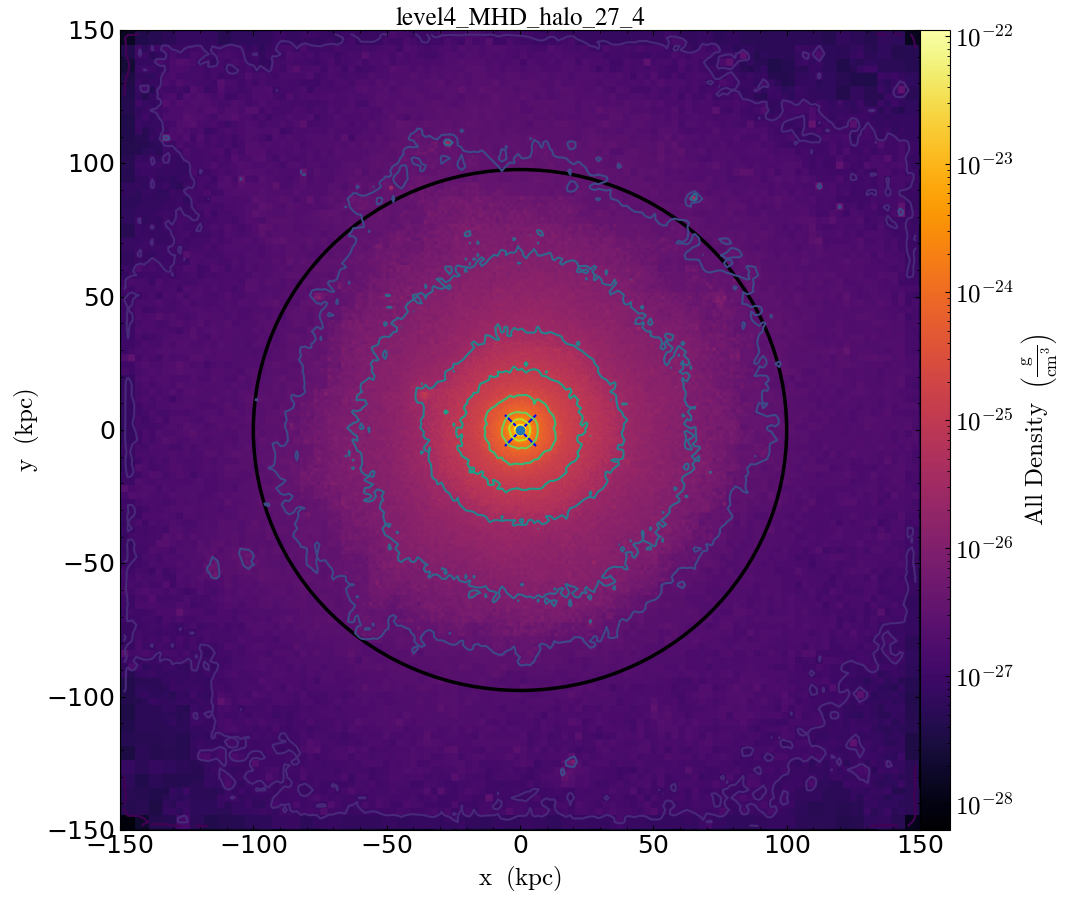
\includegraphics[width=0.5\columnwidth]{./pics/MHD_Vs_DM/level4_MHD_halo_27_outter.png}}
  \caption{DM density for inner (left) and outer (right) parts of the halo 27. We present both versions: DM (up) \& MHD (down). The horizontal and vertical axes are aligned to the major and medium semi-axes respectively. Here, it is evident that this halo is more spherical at bigger radii and more triaxial at the central parts. }
  \label{fig:slices}
\end{figure}

To graphically illustrate this process, in figures \ref{fig:slices}, we present a halo in which this rounding effect is evident for both degrees of realism: DM-only and MHD. However, to eliminate any possible qualitative bias, on figure \ref{fig:DM_MHD} we present a quantitative version of this effect. There, we include all axial ratios, which clearly become closer to 1 for bigger radii. \\

Additionally, on figure \ref{fig:DM_MHD}, we include a quantification of the triaxiality, namely $T=\frac{1-b/a}{1-c/a}$. This measurement $T$ tends towards unity when the medium-to-major axis ratio becomes equal to the minor-to-major ratio, i.e. when the halo becomes prolate. When the medium axis is close to the major axis but not to the minor axis, $T$ tends to a null value, i.e. when the halo exhibits an oblate shape. In these terms, halos are expected to be more prolate on the inside and more oblate on the outside. Even though the perfect spherical shape has a divergent/undefined $T$ value, prolate shapes are associated with triaxial characterizations and oblate shapes are identified as approximately spherical shapes. \\

In DM halos, the tendency of axial ratios $(b/a,c/a)$ towards unity in figure \ref{fig:DM_MHD} is clearly monotonic for $r>$1Kpc (see also the triaxiality parameter T). However, for MHD halos this is not the case. Phenomenologically MHD halos tend towards more spherical shapes at $r>$1Kpc until some axisymmetry is reached around $10-50$Kpc (see minimum of triaxiality parameter T). In other words, for DM halos we can say that the axial ratios $(b/a,c/a)$ are always locally increasing whereas for MHD halos, we can only surely state that these axial ratios increased overall in the range $1-100$Kpc, that is, this rounding effect is global and not necesarily true when sampled locally at a specific radius. \\

\begin{figure}
\centering
\subfloat[halo 16]{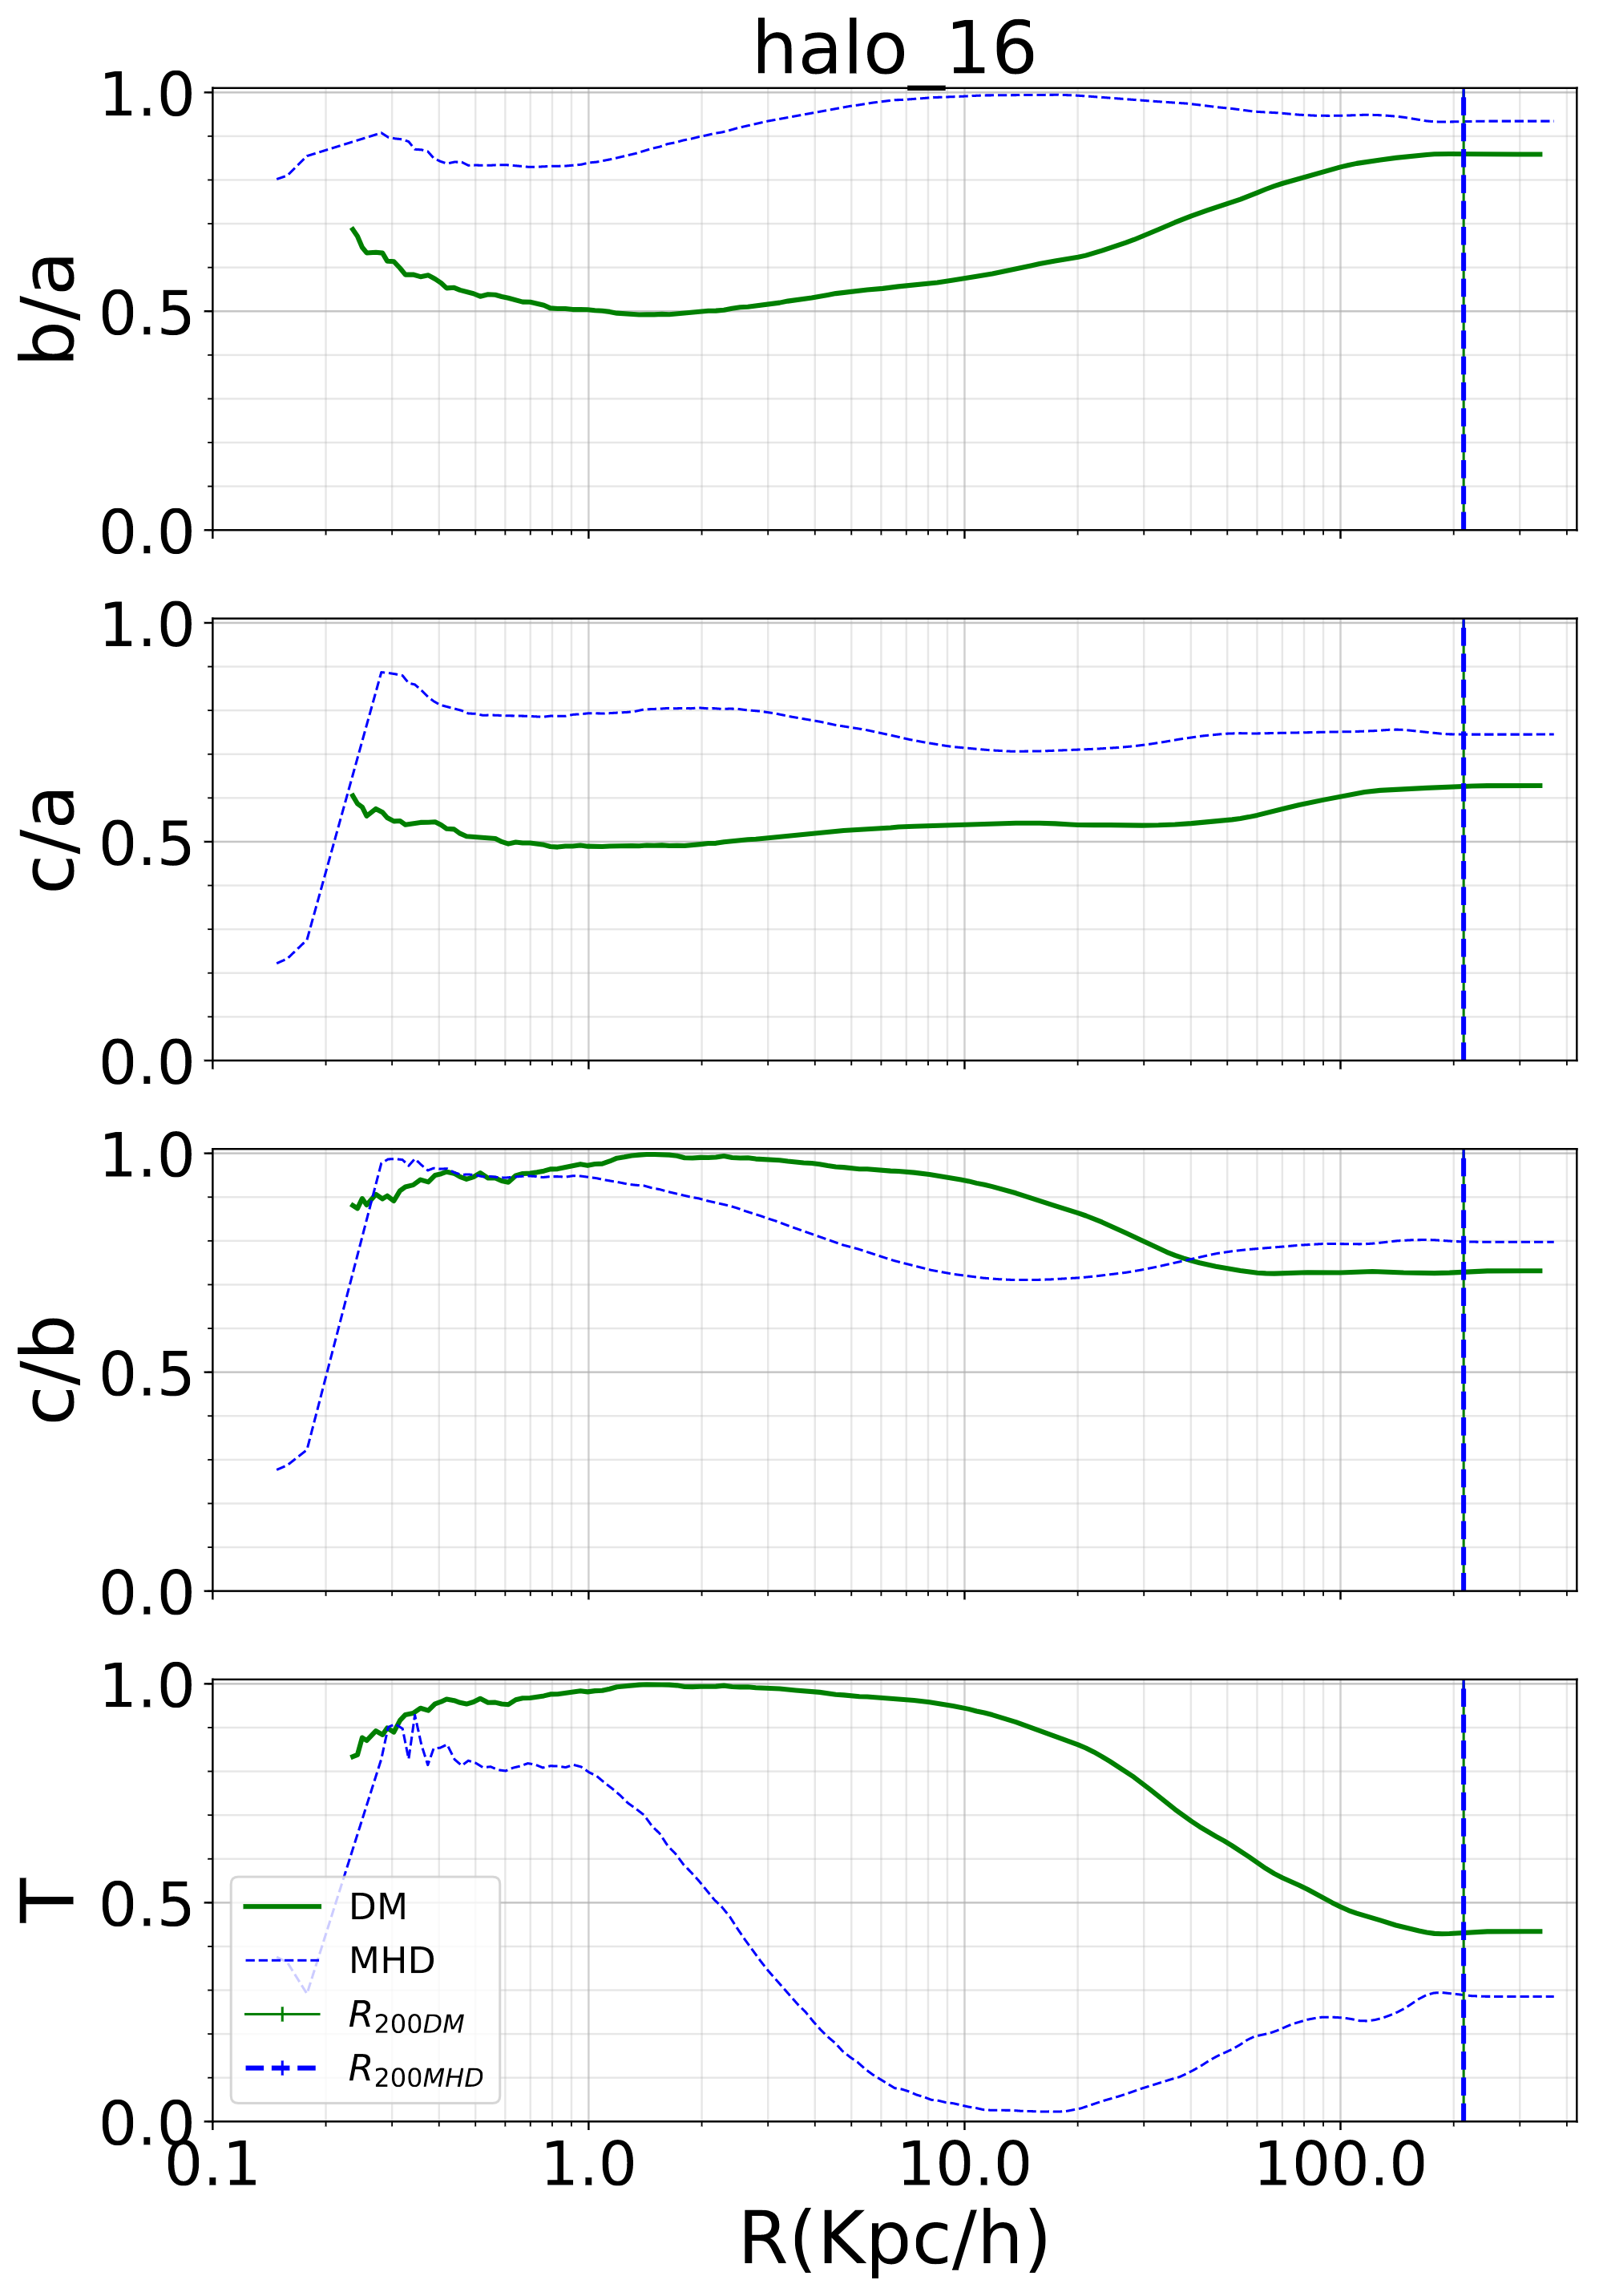
\includegraphics[width=0.5\columnwidth]{./pics/halo16.png}}
  \hfill
  \subfloat[halo 27]{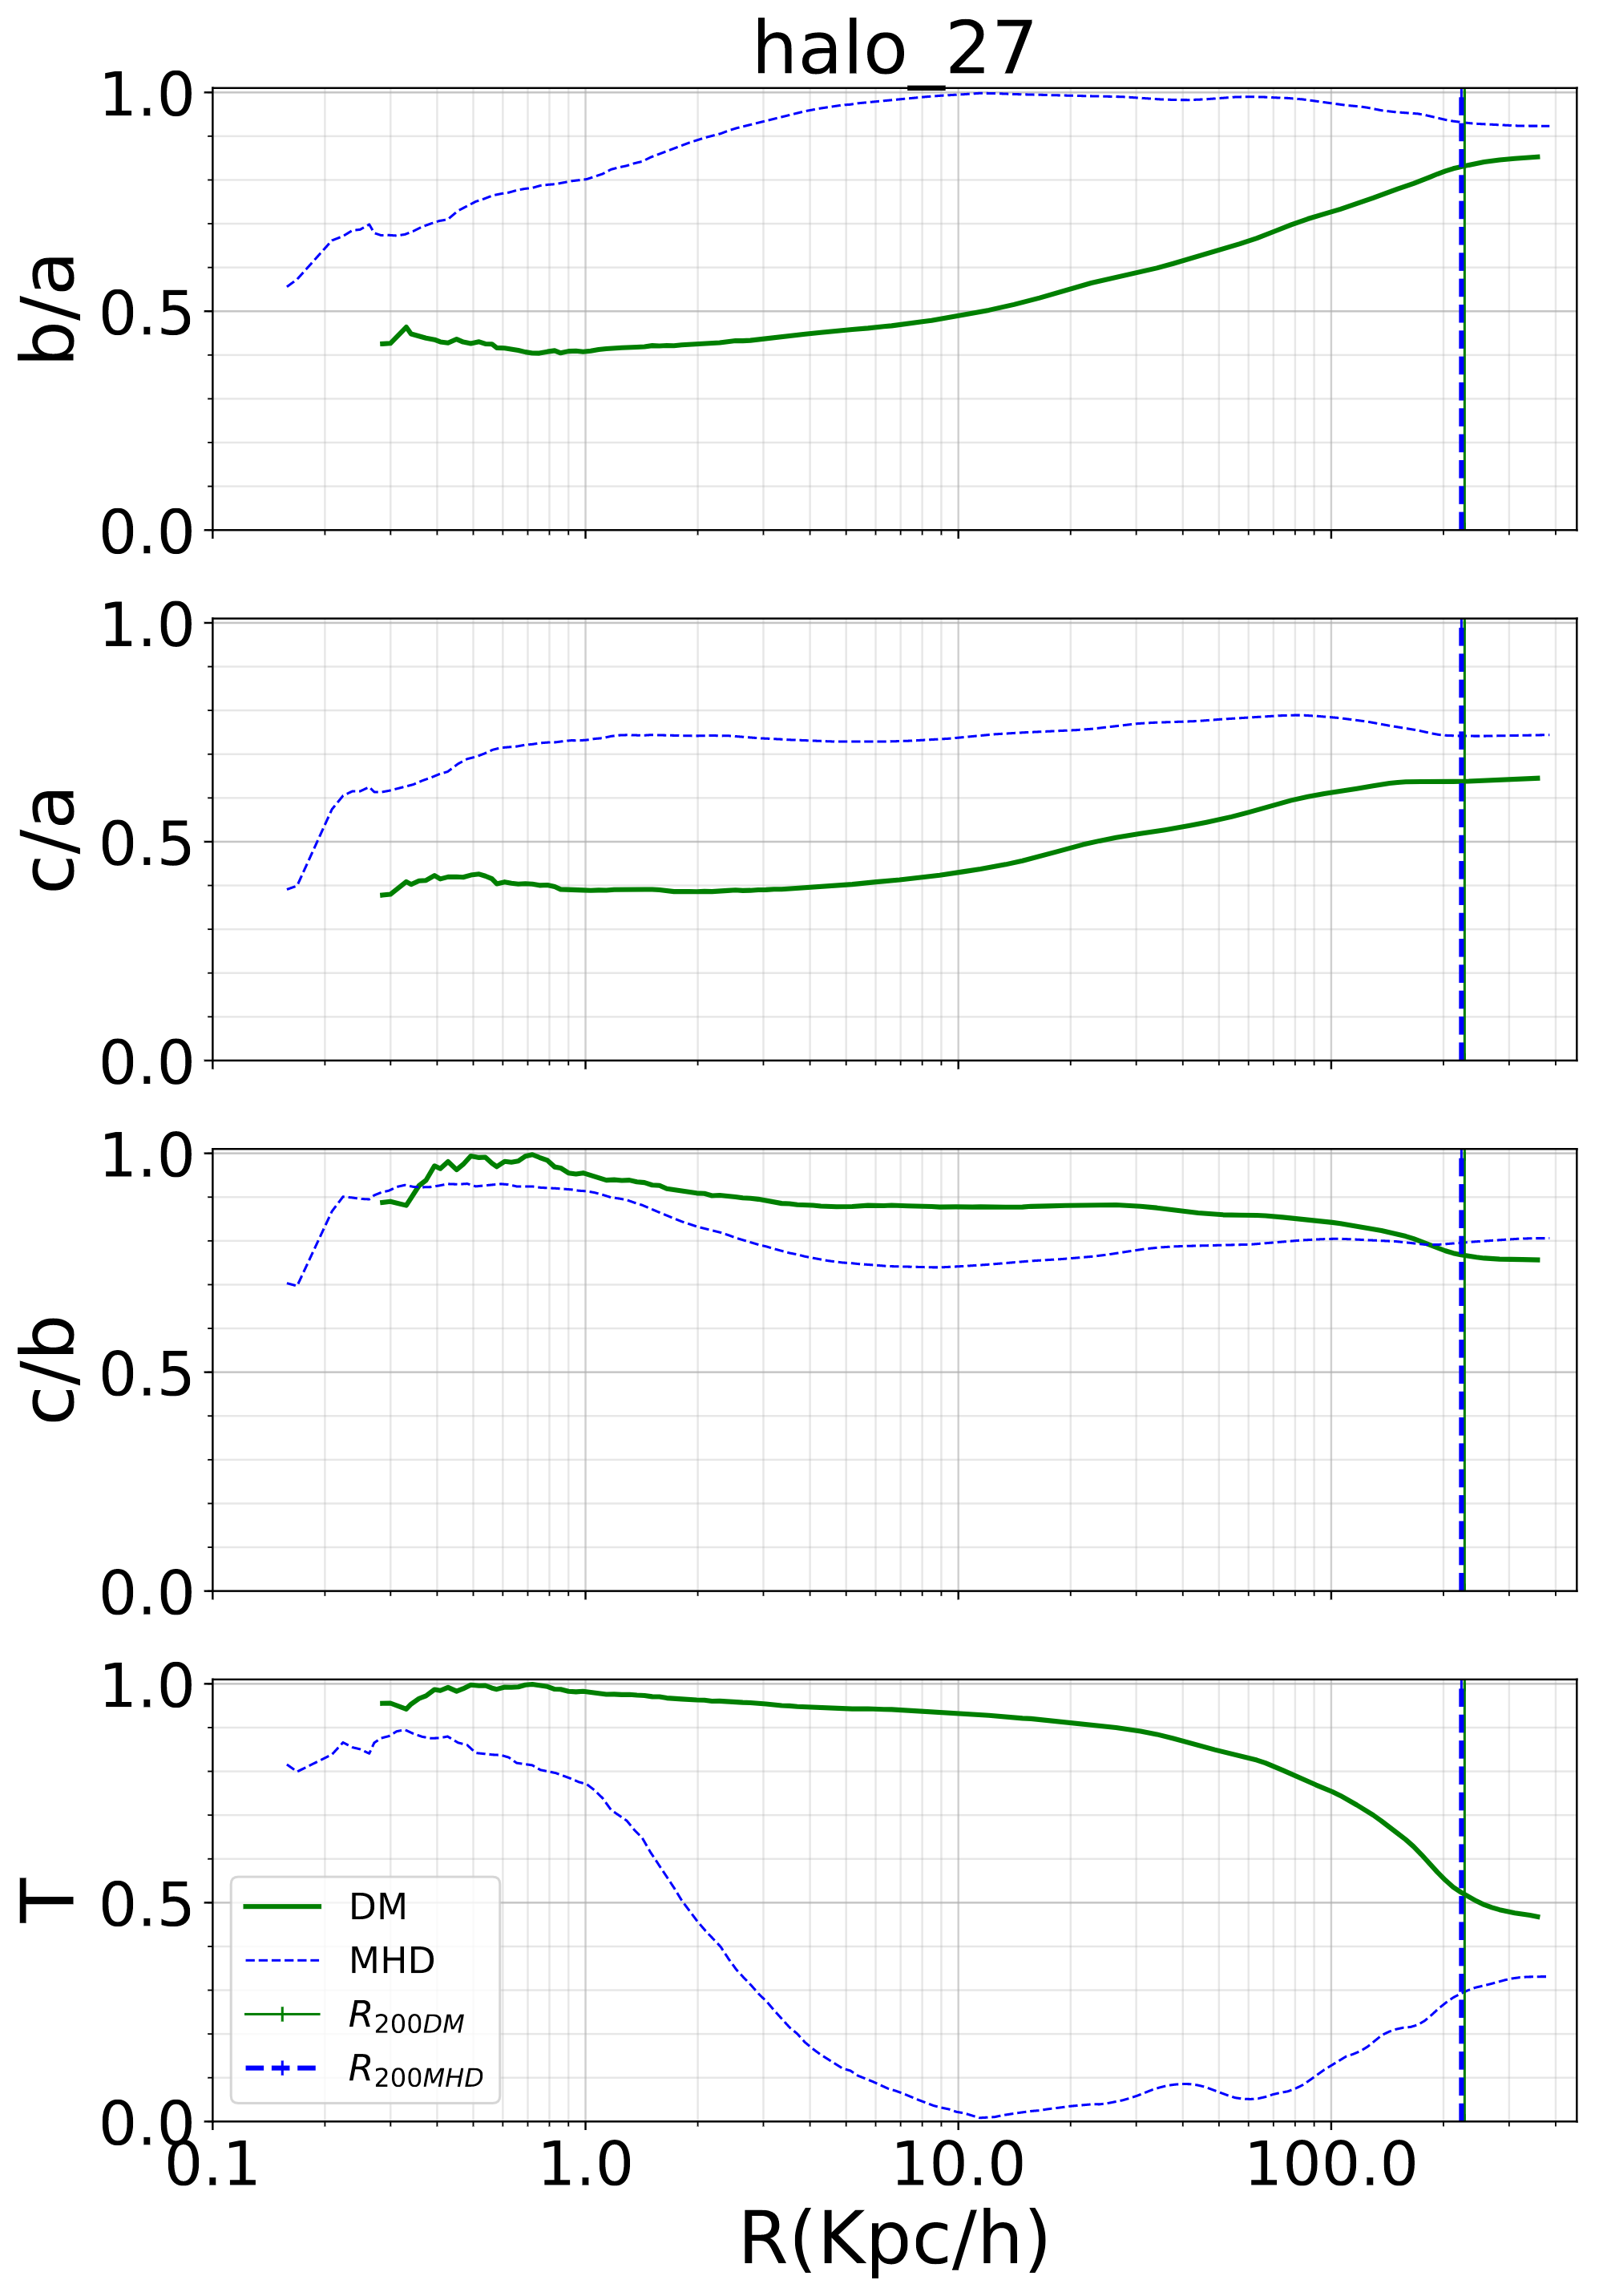
\includegraphics[width=0.5\columnwidth]{./pics/halo27.png}}
\caption{Radial profile for axial ratios and the triaxiality parameter $T=\frac{1-b/a}{1-c/a}$ from halo 27 and halo 16. These halos have a clear radial tendence towards sphericity (for smaller radii until $\approx 3$Kpc), which can be confirmed with the triaxiality parameter. }
\label{fig:DM_MHD}
\end{figure} 


This rounding effect with radius can be better illustrated on the triaxial $c/a$  Vs  $b/a$ plane where we may also note that this is in fact a global tendency for all halos.\\
In figure \ref{fig:Triaxiality_Inner_Outer}, we show the axial ratios on the plane $c/a Vs b/a$. There, each dot labeled by radius represents a specific shape. In this plane, oblate halos are represented by the vertical line $x = 1$, prolate halos are identified on the identity line and spheres are exactly the point $(1,1)$. This gives us a broader idea of the evolution of the shape. The tendency is clear for halos to get rounder with increasing radius. In fact, the difference in shape clear enough that it is possible to identify groups in case the radius label is hidden.\\

\begin{figure}[!ht]
  \centering
  \subfloat[Level4 DM inner Vs outer regions]{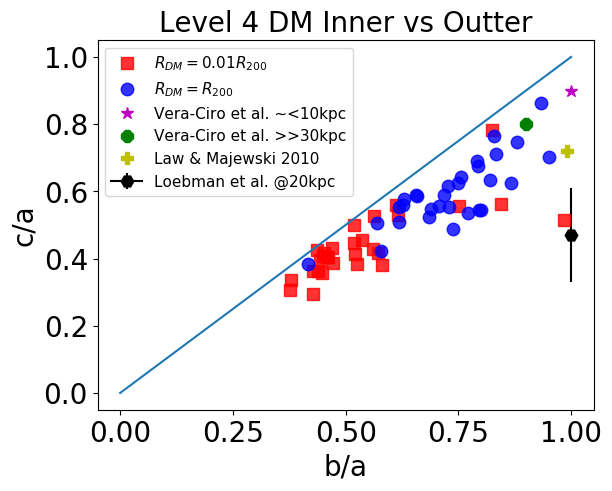
\includegraphics[width=0.5\columnwidth]{./pics/Triaxial_Plane/Triaxiality_DM_lvl4.png}}
  \hfill
  \subfloat[Level4 MHD inner Vs outer regions]{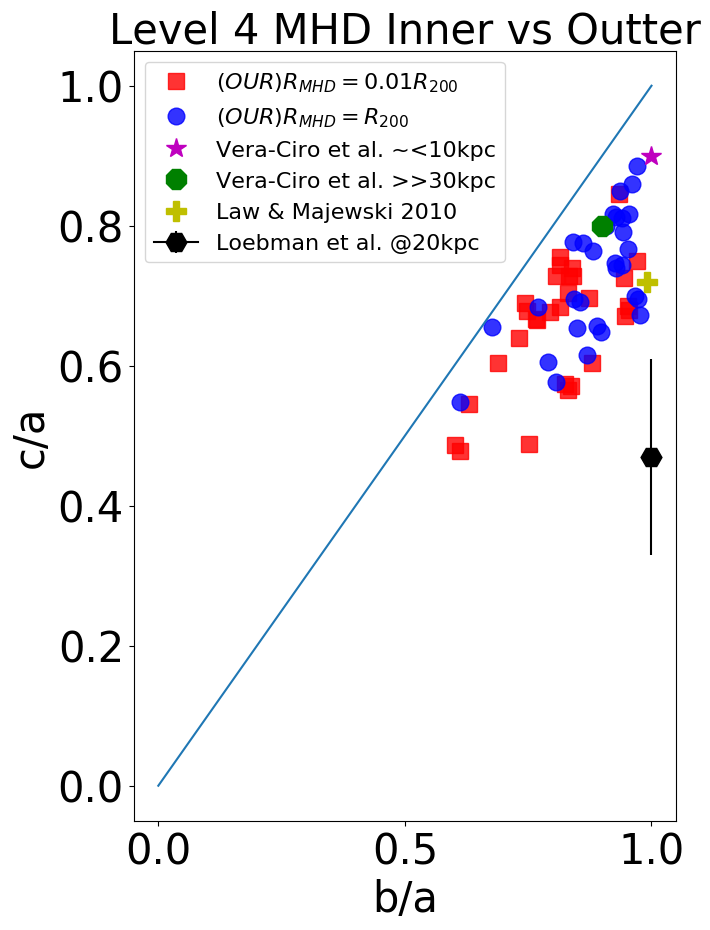
\includegraphics[width=0.5\columnwidth]{./pics/Triaxial_Plane/Triaxiality_MHD_lvl4.png}}
  \hfill
  \caption{General tendency on the triaxial plane $c/a$ Vs $b/a$. Some observational constraints are plotted alongside our results}
    \label{fig:Triaxiality_Inner_Outer}
\end{figure}

\subsection{The effect of gas on the halo shape}
We have simultaneously corroborated the rounding effect of radius on the halo shape from DM-only and MHD simulations. However, from the parallel presentation of results from MHD and DM simulations in previous figures \ref{fig:DM_MHD,slices}, it is also noticeable that MHD halos are in general more spherical than DM halos, which is to be expected from the presence of baryons\cite{Barnes_and_Hernquist_1996,Springel_et_al._2004,Bryan_et_al._2013}.\\

 Unlike DM, gas collapses and generates disks which are much denser than the DM structures. This amplifies the scattering effect of the gravitational potential and represents a strong source of axisymmetry that may shape the DM particle orbits. iI we apply the same logic as before, we would expect that the inner regions of the halo are more spherical where there is presence of baryons, that is, at the glactic disk regime. We expect the same for outer regions but this effect is predicted to be less significant due to the weaker effect of the gravitational potential of the axisymmetric baryonic disk.\\

For instance, recurring again to the figures \ref{fig:slices}, now comparing the graphics vertically, the rounding effect of visible matter is clear. For a more quantitative illustration of this, we can refer the axial ratios in figure \ref{fig:DM_MHD}. \\

\begin{figure}[!ht]
  \centering
  \subfloat[Level4 MHD Vs DM at inner regions]{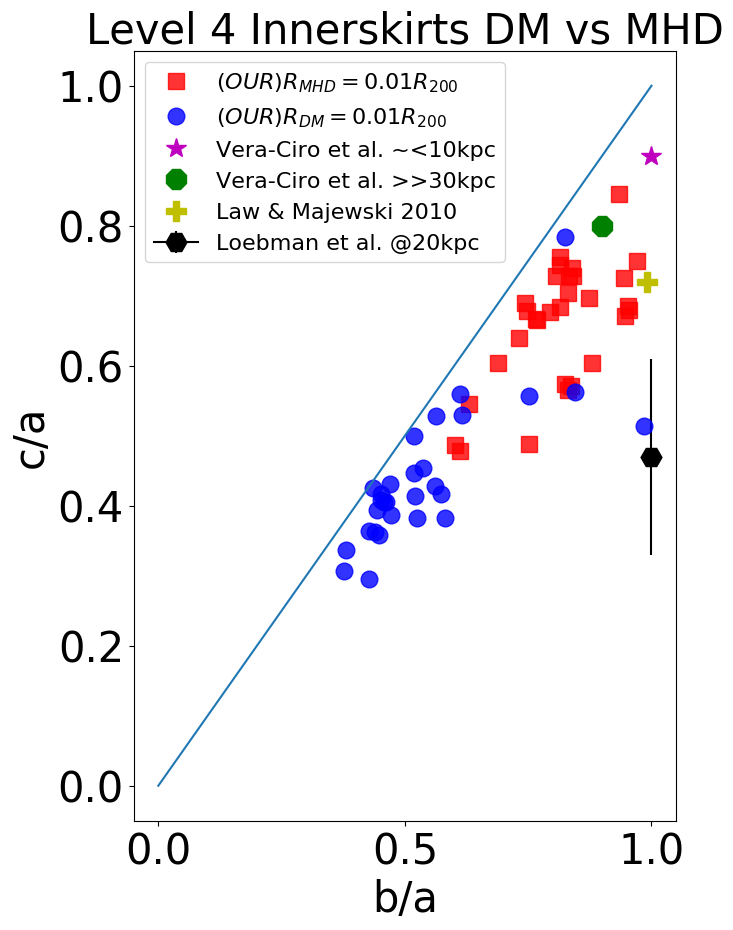
\includegraphics[width=0.5\columnwidth]{./pics/Triaxial_Plane/Triaxiality_Inner_lvl4.png}}
  \hfill
  \subfloat[Level4 MHD Vs DM at outer regions]{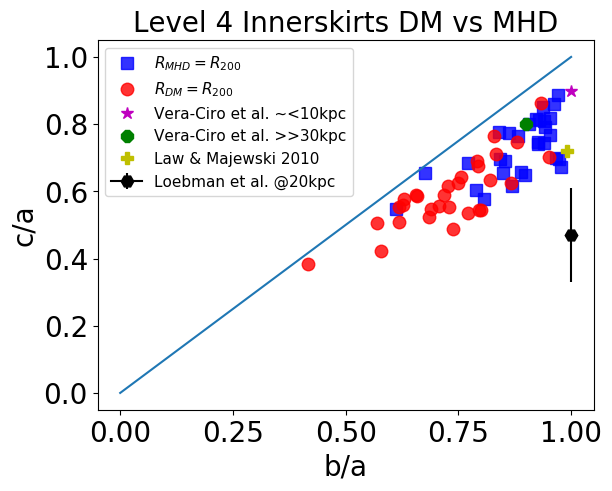
\includegraphics[width=0.5\columnwidth]{./pics/Triaxial_Plane/Triaxiality_Outter_lvl4.png}}
  \hfill
  \caption{Axial ratios as shown on $c/a$ Vs $b/a$. Each dot represents a halo shape at some radius. Some observational constraints are plotted alongside our results. Here, dots are clustered, proving the general tendence of halos to get rounder on the outer parts. }
    \label{fig:Triaxiality_DM_MHD}
\end{figure}

From previous pictures it is evident that the presence of baryons affects the halo shape by making it rounder, and it is also clear that this effect is amplified around $10-50$Kpc (see the behaviour of the triaxiality parameter T). To confirm this effect taking into account all 30 simulated halos, we recur again to triaxiality plane on \ref{fig:Triaxiality_DM_MHD}, where the tendency becomes evident.\\

So far, our results are in accordance with previous work. Nonetheless, in the specific case of MW-like galaxy simulations, we have confirmed the expected tendency in an unprecedented statistically significant sample of 30 galaxies from Auriga, compared to the 4-sample galaxies from the previous state-of-the-art Aquarius simulations. Moreover, we confirmed that these results are sustained for the specific case of novel MHD MW-like galaxy simulations where we could also analyze the effect of baryons on the DM halo shape.\\

\section{Historical shape}
Taking into account the previous phenomenology for halo formation, it is possible to extend 
its reach for the analysis of the historical evolution of the halo shape.\\

Given that the DM halo particles are constantly subject to the scattering effect of the inner potential, we expect that with time, at every radii, the cumulative scattering events are more numerous. Consequently, we expect a systematic rounding effect of the halo shape with time driven by the randomization of DM particle objects through the process of scattering. Furthermore, given that the cross-section of the halo gets bigger at bigger radii, we expect that this rounding effect with time is more significant at outer shells, specially where the accretion of matter occurs.\\

% Recalling that inner shells of the halo are isolated from the gravitational effect of outer shells, the only significant source of disruption in time of this radial regime are external structures that perform some torque on them. Outer shells must feel this source of deformation too in addition to the effect from the inner gravitational potential. Consequently, we expect a systematic change on the halo shape with time, which becomes more significant for bigger radii.\\
 
Major events like mergers, may completely disturb a galaxy shapes and erase any memory that it may keep with time. However, from $z\approx 1$ onwards, these events are very rare \cite{Tormen_et_al._1998} and we expect that any source of disruption is weak and is reduced to the previously mentioned factors. \\  

\begin{figure}[!ht]
  \centering
  \subfloat[halo 16 DM]{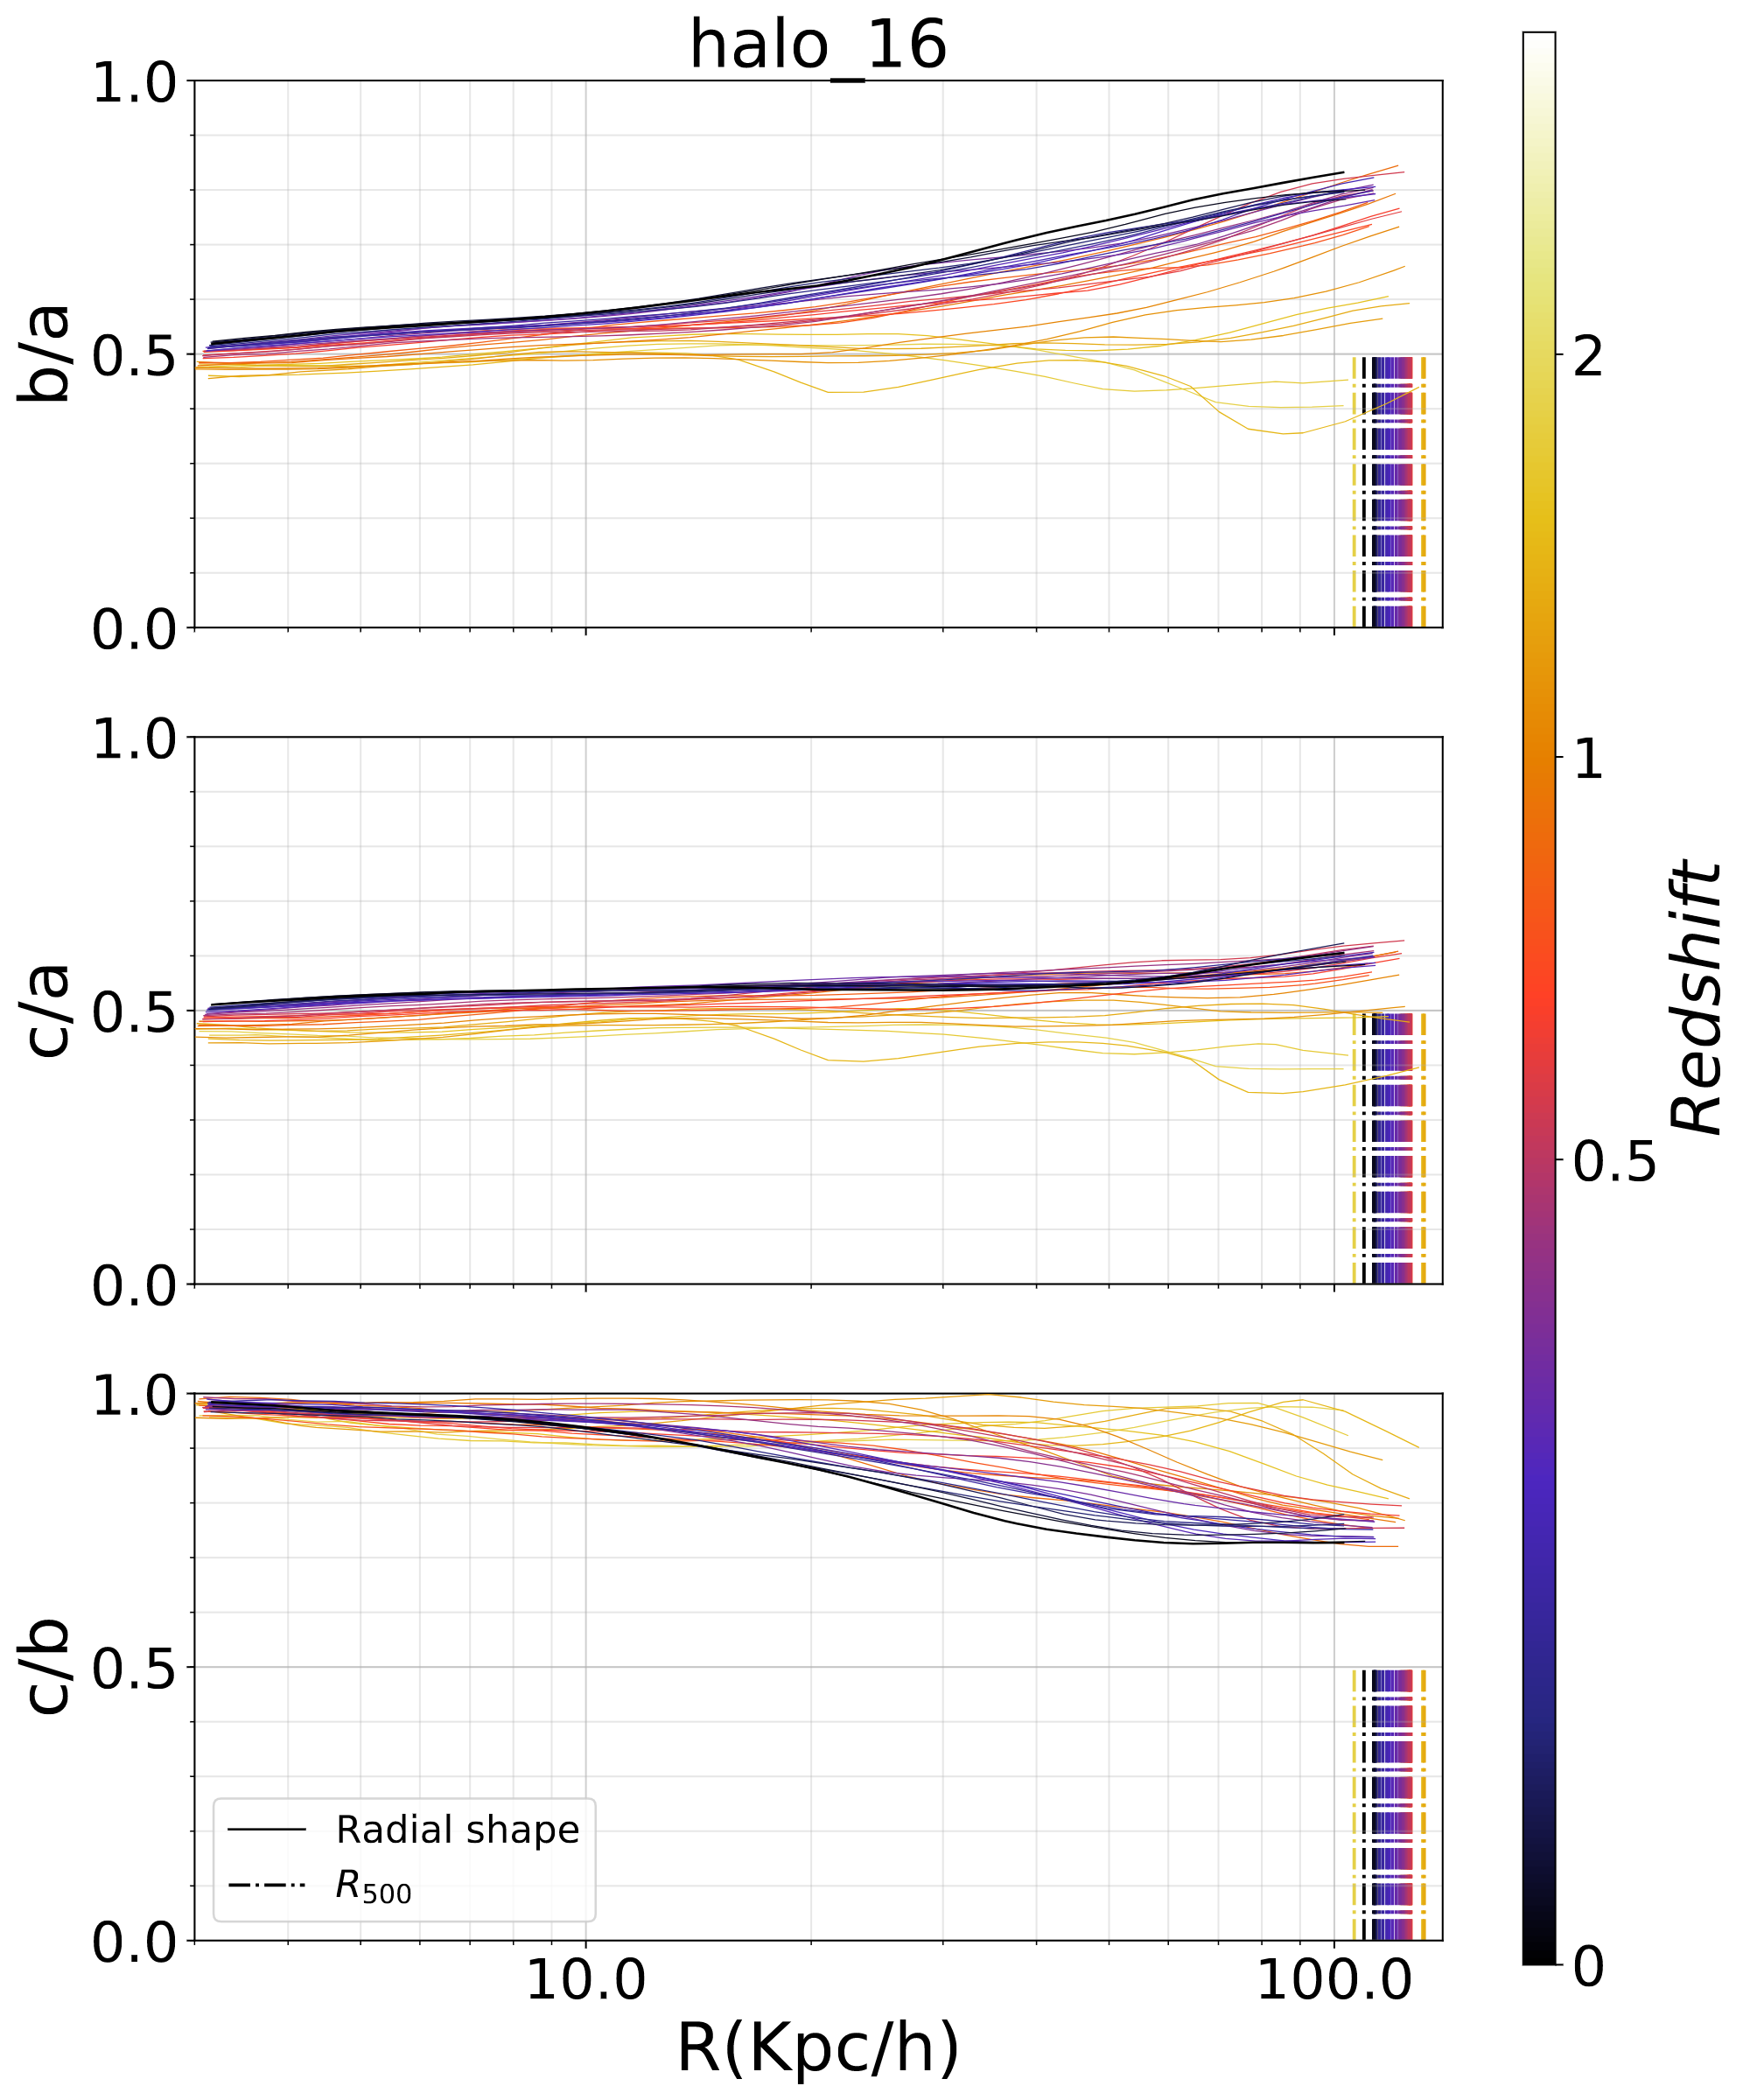
\includegraphics[width=0.5\columnwidth]{./pics/Redshift/halo_16_level3_DM_Z.png}}
  \hfill
  \subfloat[halo 16 MHD]{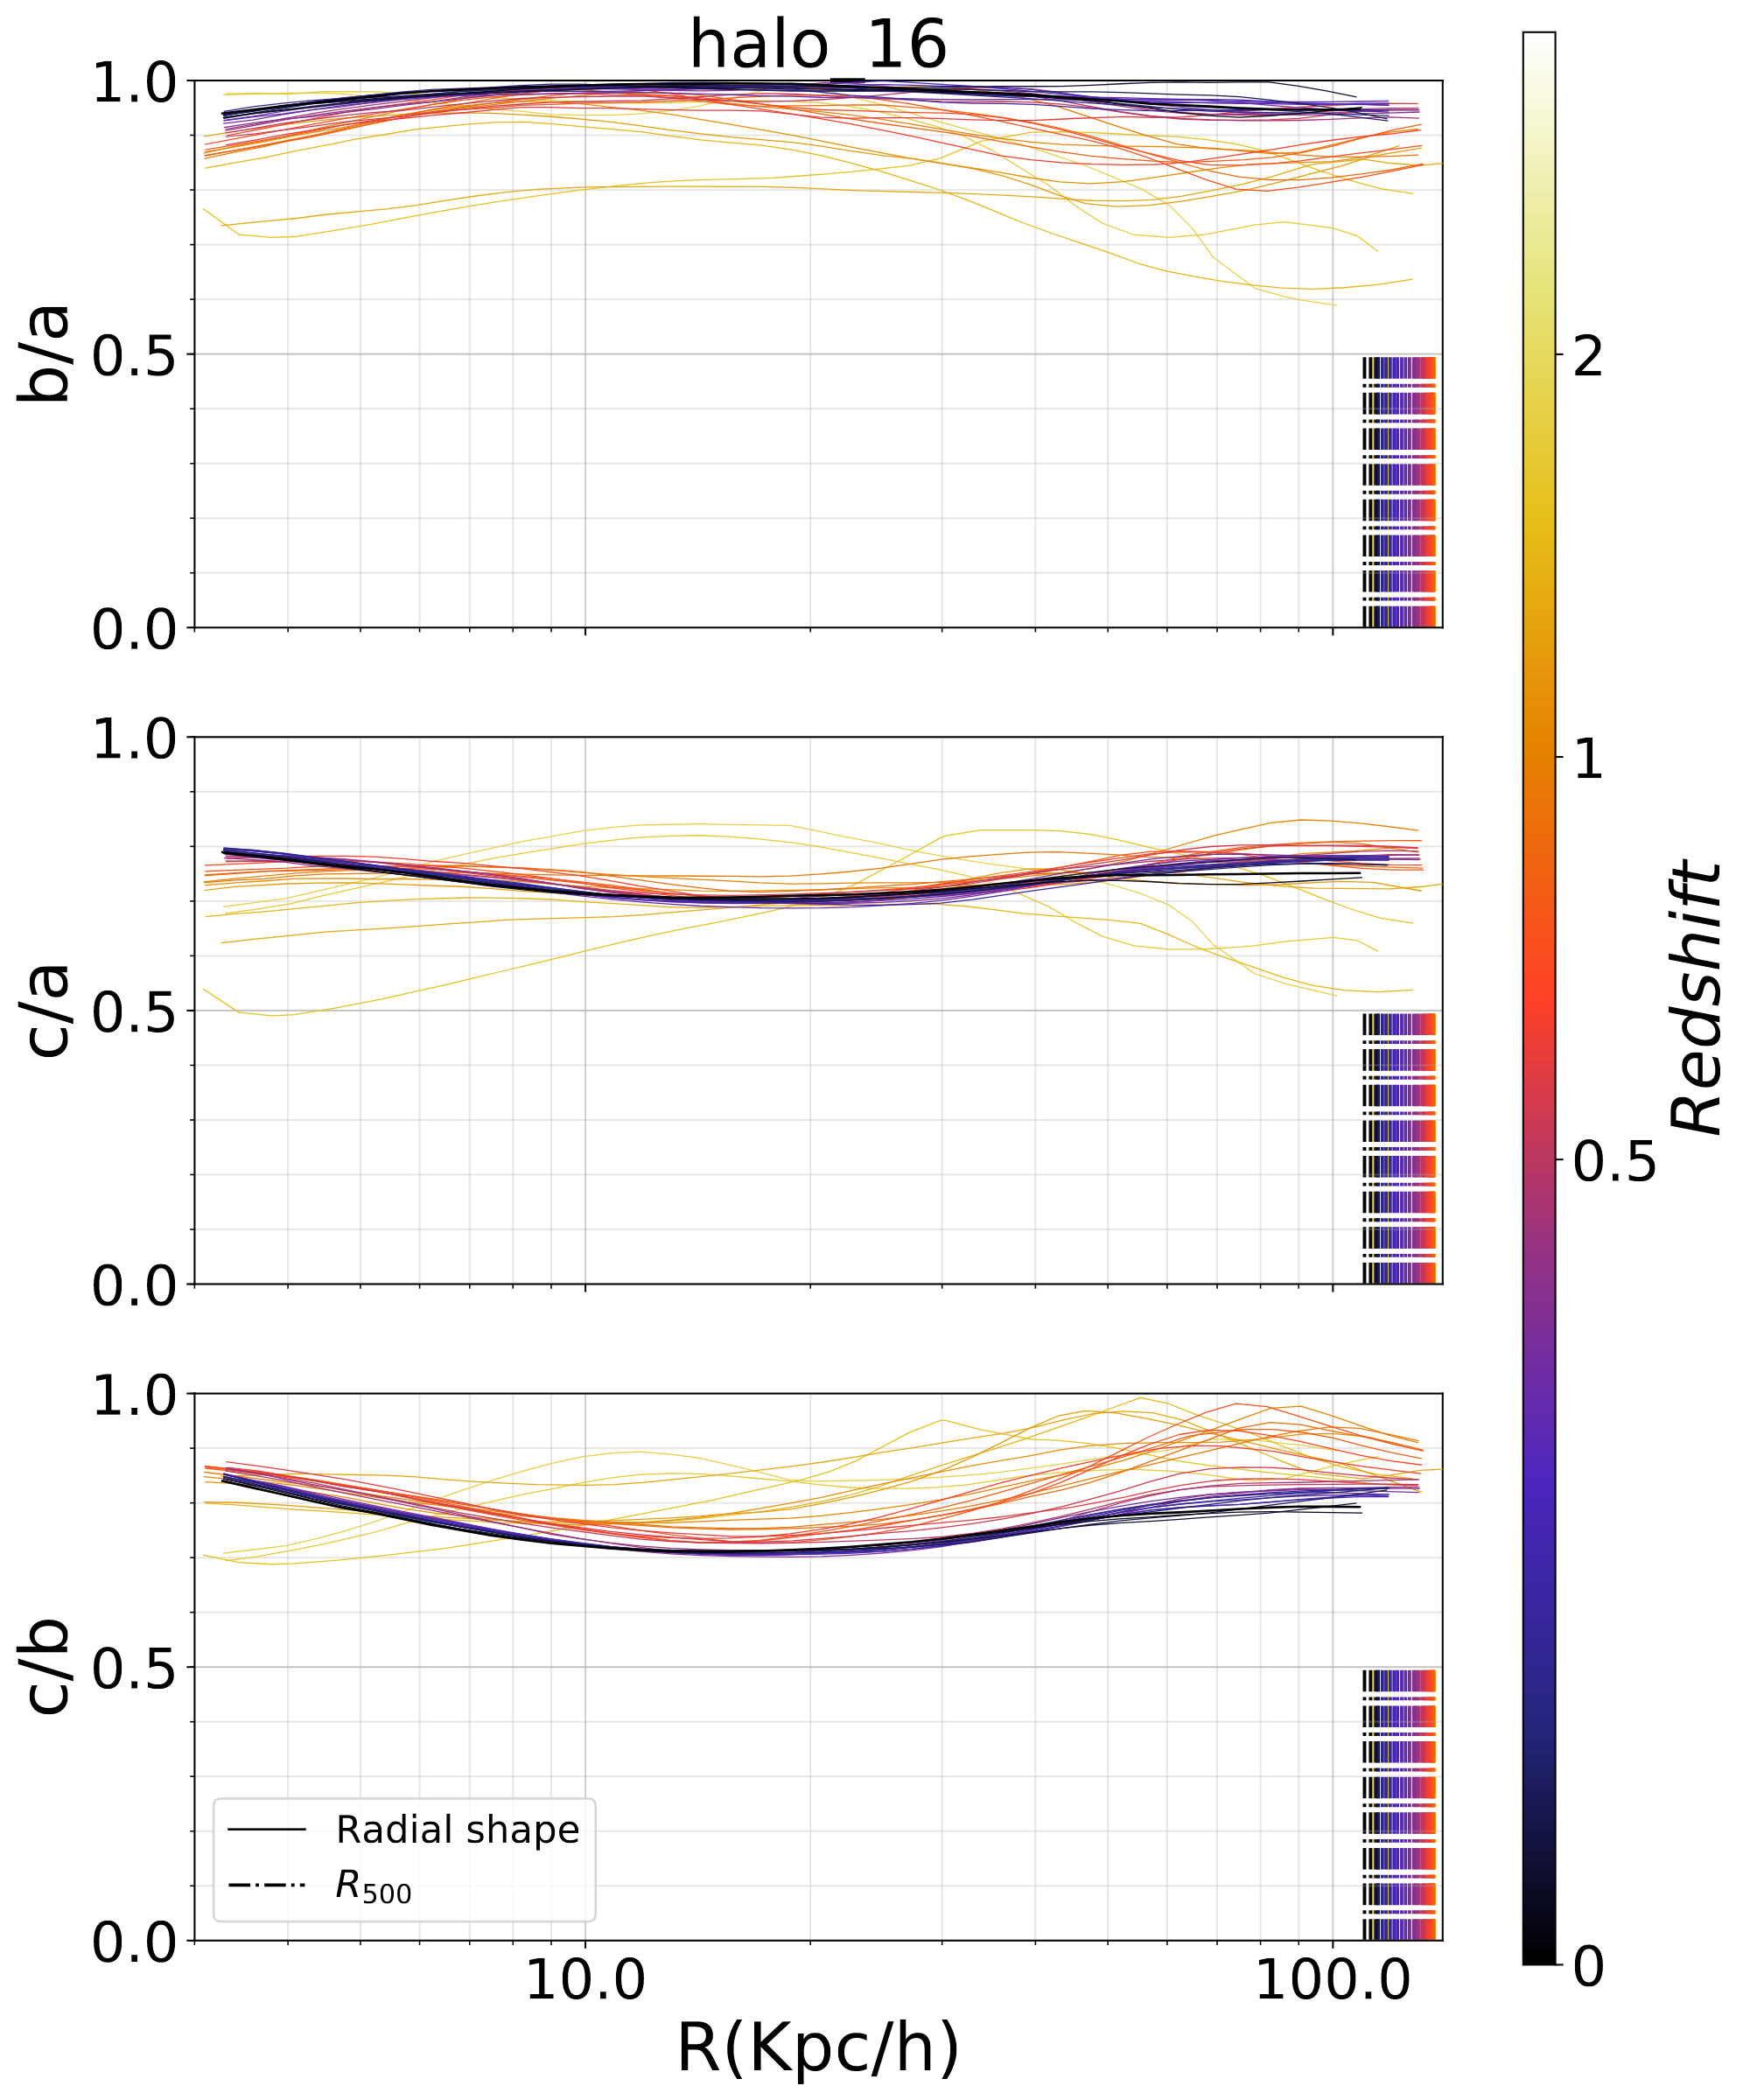
\includegraphics[width=0.5\columnwidth]{./pics/Redshift/halo_16_level3_MHD_Z.png}}
  \caption{Radial profile (comoving) of axial ratios for halo 16 in terms of redshift (color). This halo maintains its shape until $z\approx 1$ obviating the systematic rounding effect in time from scattering potentials. }
  \label{fig:RedshiftGood}
\end{figure}

In figures \ref{fig:RedshiftGood} we present the evolution of the radial profile of the shape of a halo that managed to conserve its integrity until $z \approx 1$. In this case, we show our results in terms of the comoving coordinates to obviate the scale factor and make these profiles comparable. The halo becomes systematically and monotonically more spherical as it evolves in time, being this effect more relevant for $r>50Kpc$.\\

In figures \label{fig:RedshiftDMbad} we present a specially rare case of a halo that was perturbed at some time around $z\approx 0.5$. This perturbation is specially evident because of the discontinuity caused in the radial profile and the large differences in the virial radii. \\  


\begin{figure}[!ht]
  \centering
  \subfloat[halo 21 DM]{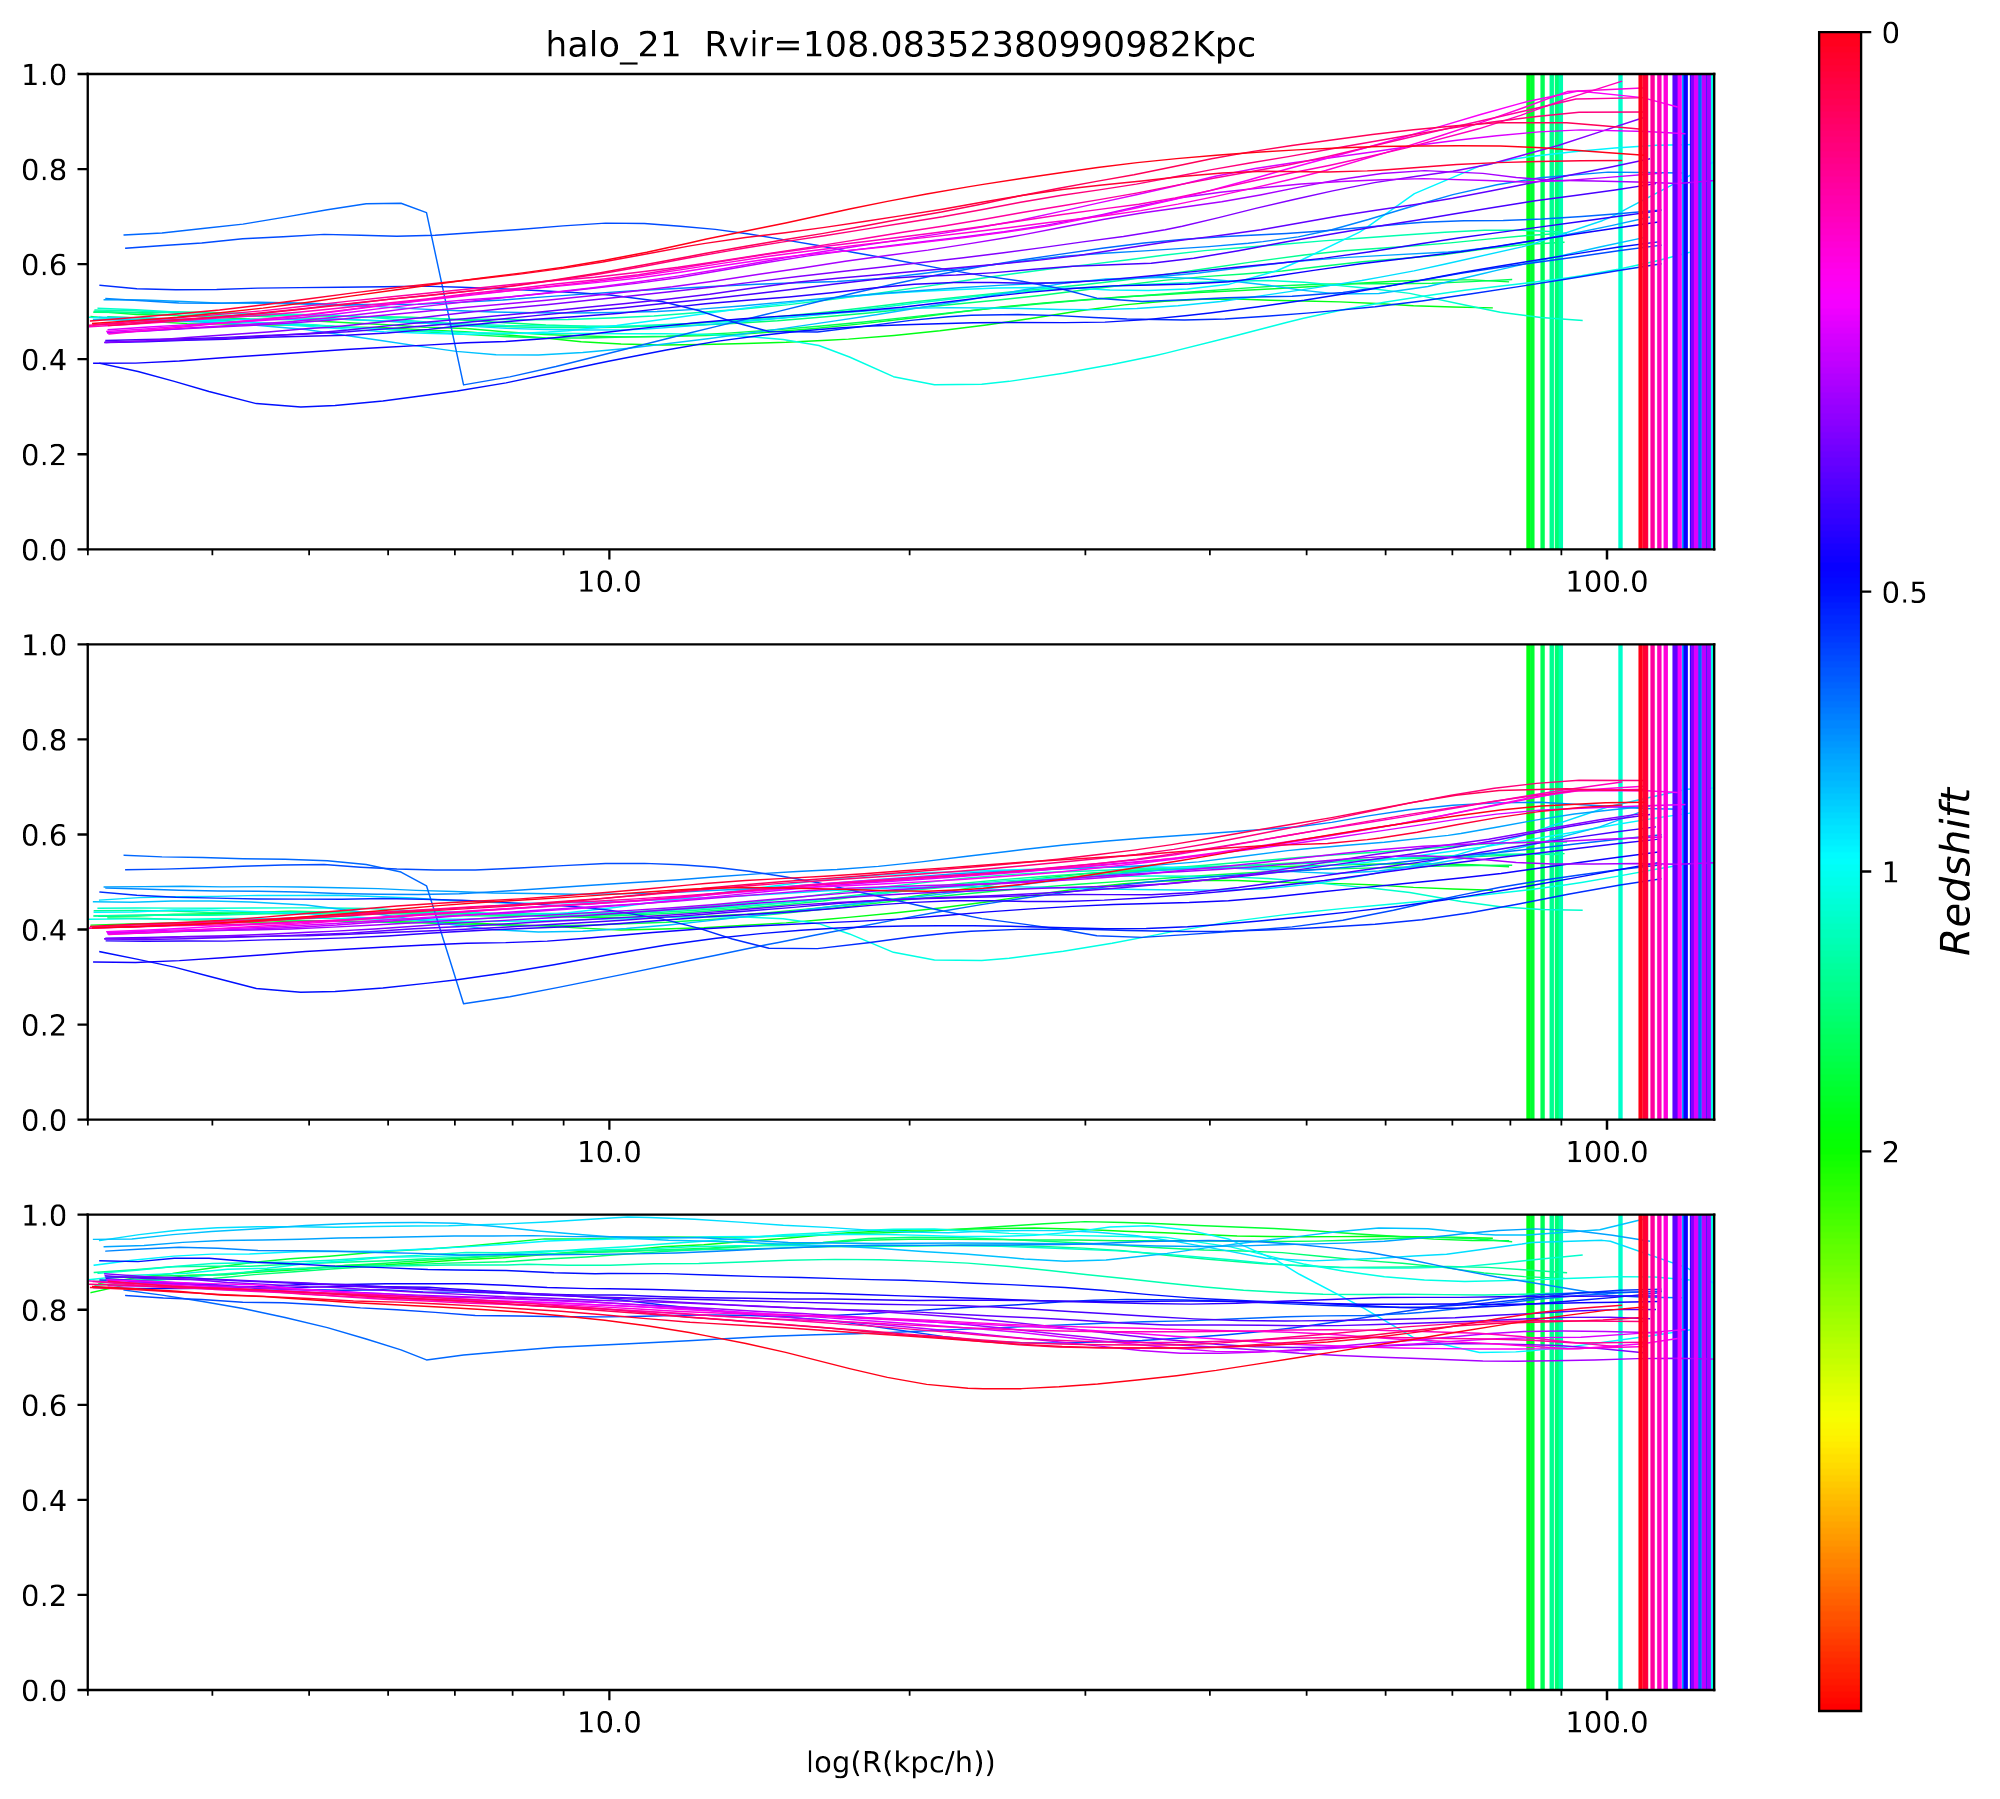
\includegraphics[width=0.5\columnwidth]{./pics/Redshift/halo_21_level3_DM_Z.png}}
  \hfill
  \subfloat[halo 21 MHD]{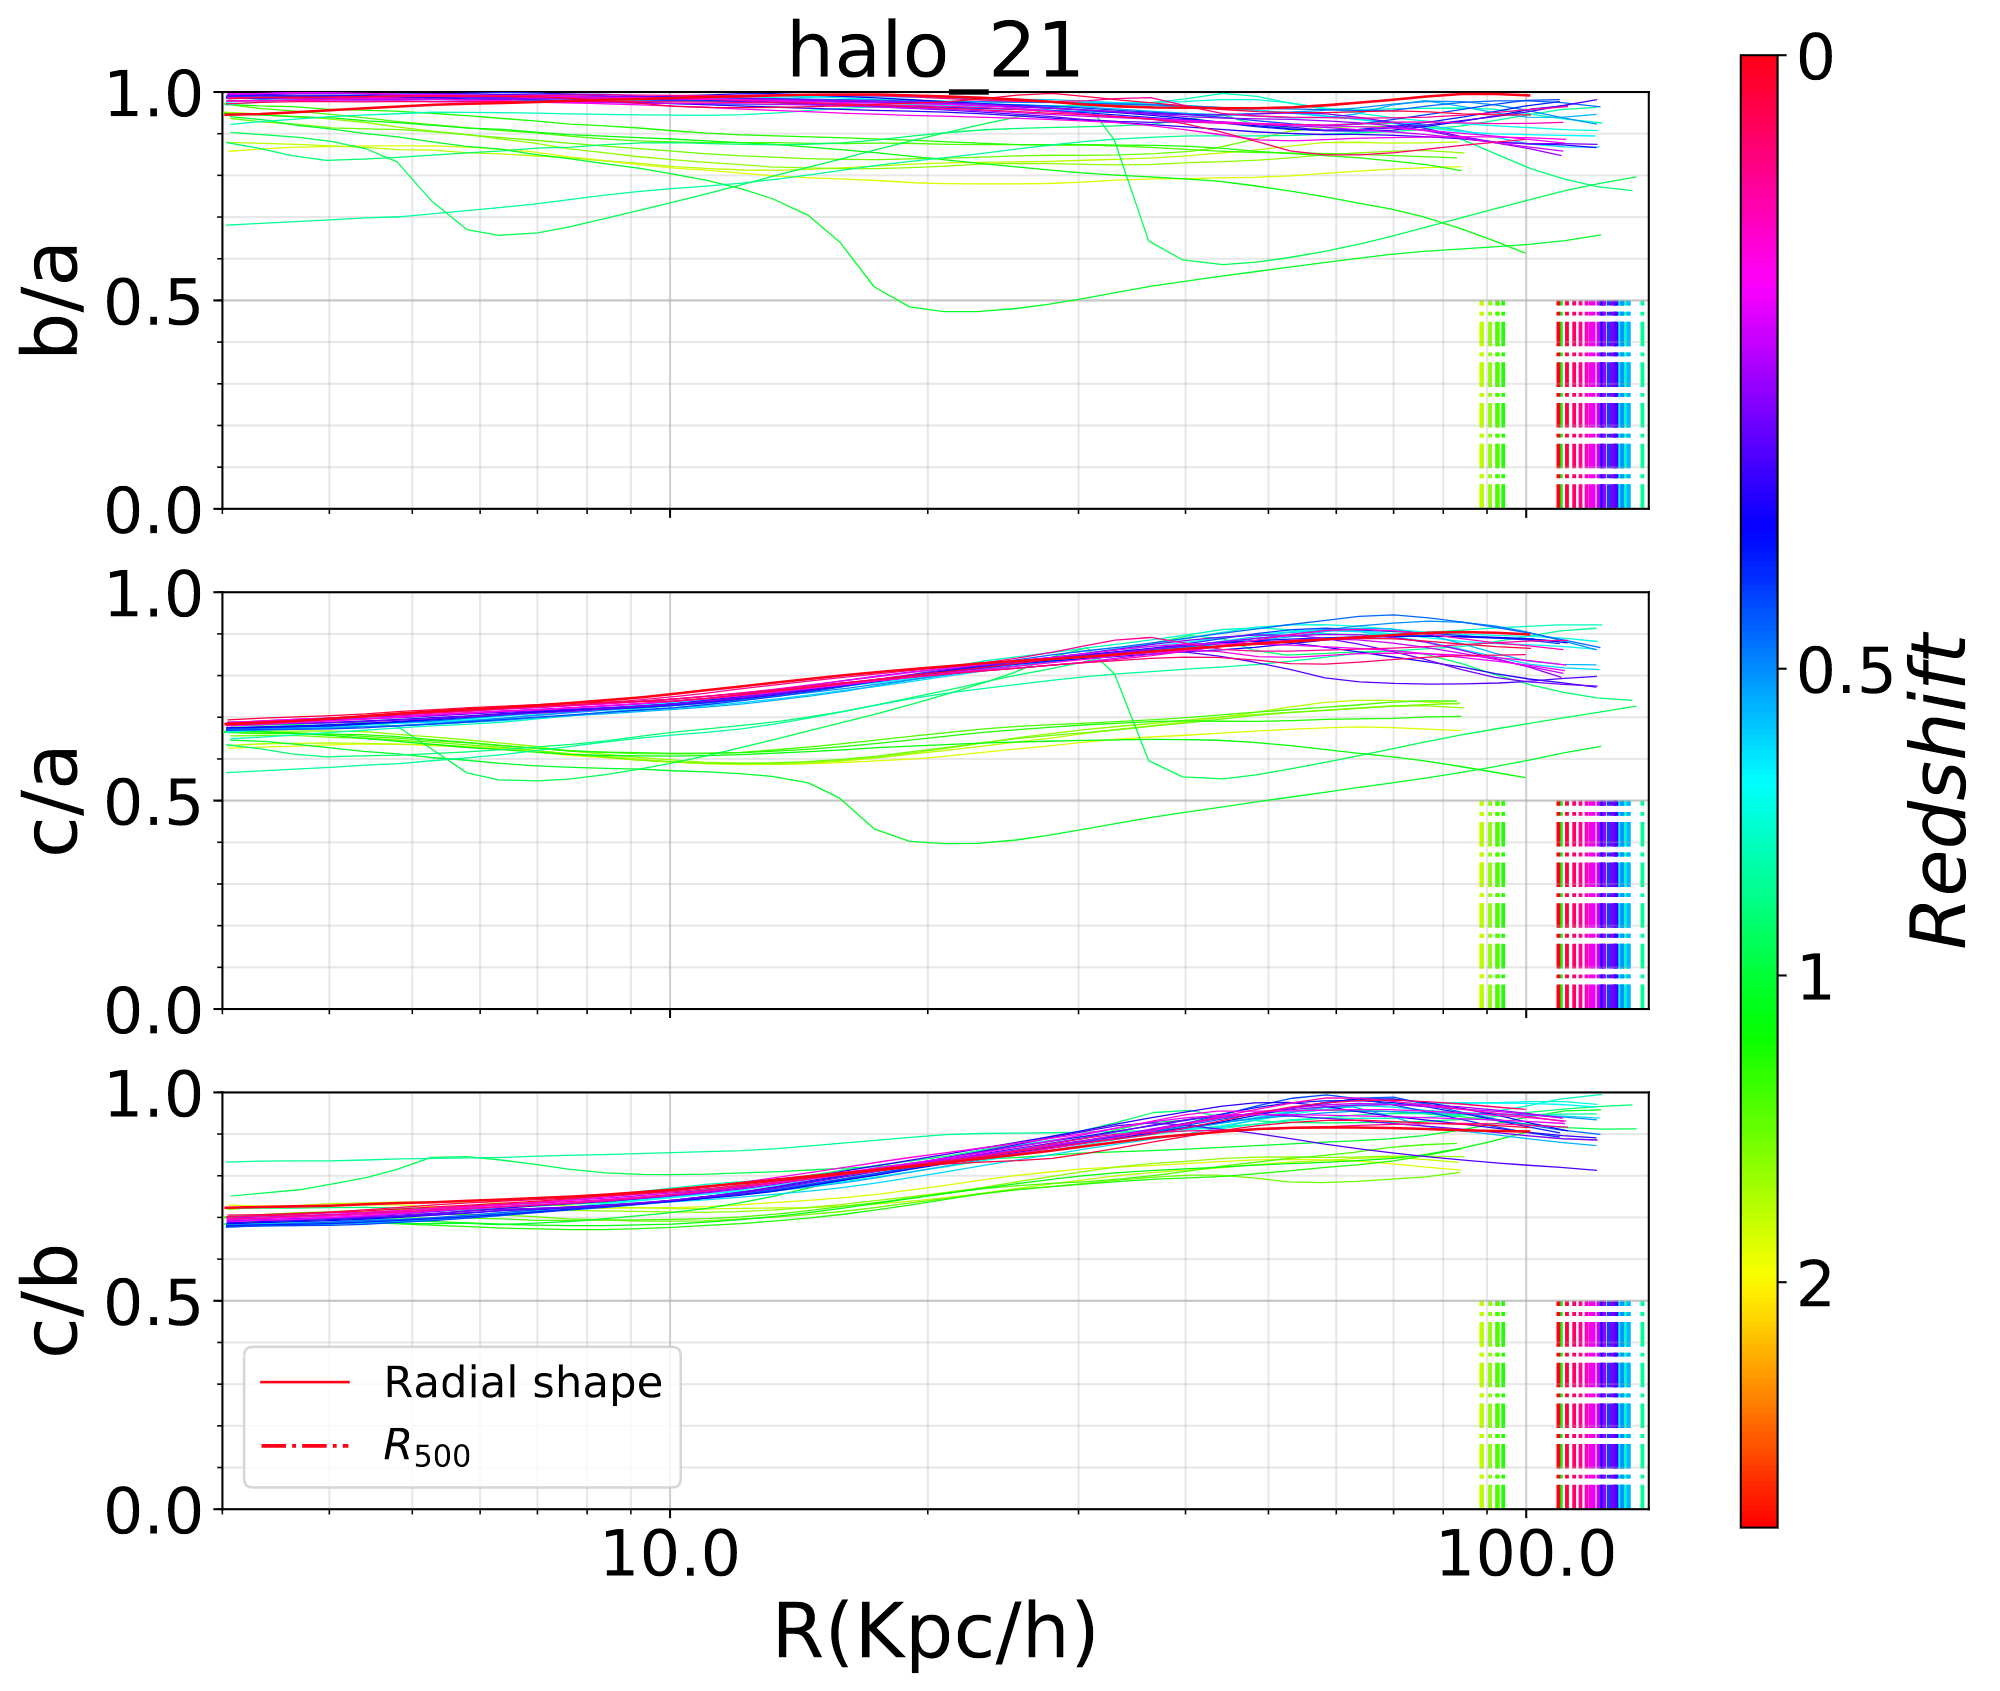
\includegraphics[width=0.5\columnwidth]{./pics/Redshift/halo_21_level3_MHD_Z.png}}
  \caption{Radial profile (comoving) of axial ratios for halo 21 in terms of redshift (color). This halo is disrupted around $z \approx 0.5$ which results in a certain loss of its shape memory.}
  \label{fig:RedshiftBad}
\end{figure}

Now, these results compare radial profiles in comoving coordinates, but in real life we have physical coordinates. In this order of ideas, we can state this preservation of the shape (obviating the rounding effect) without recurring to comoving comparisons.\\

In this case, consider a physical radius $R$ that is well-defined for each redshift, at which we are going to perform our historical measurements. For practical purposes let us take, for example, the virial radius at each redshift. From $z\approx 1$ onwards, mass accretion is in general steady and slow, and therefore, the virial radius will not experience significant variations in comoving coordinates. We have shown that there is a monotonical tendency for the halo to get more spherical with time at a fixed radii ($r=R_{vir}$). Furthermore, for DM-only halos, halos get monotonically rounder at bigger radii at a fixed time ($z=0$). This congruence in both tendencies can be interpreted in a congruence between the radial profile of axial ratios at redshift 0 and their historical profile at the virial radius. In other words, by sampling the axial ratios at the virial radius at each redshift, we are effectively sampling the shape for smaller radii at $z=0$. \\

To illustrate this, in figures \ref{fig:RedshiftDM} we present the historical and radial profiles of the previously analyzed halo shapes. For the halo that maintained a consistent shape during time, there is a clear correlation between the historical and radial profiles, both clearly tending to more spherical shapes at lower redshifts and bigger radii. In the case of the halo that had a major disrupting event, the fact that this correlation is not clear is an evidence of the memory loss by the massive infalling material around $z=1$.\\  

%\begin{verbatim}
\begin{figure}[!ht]
  \centering
  \subfloat[halo 16 DM]{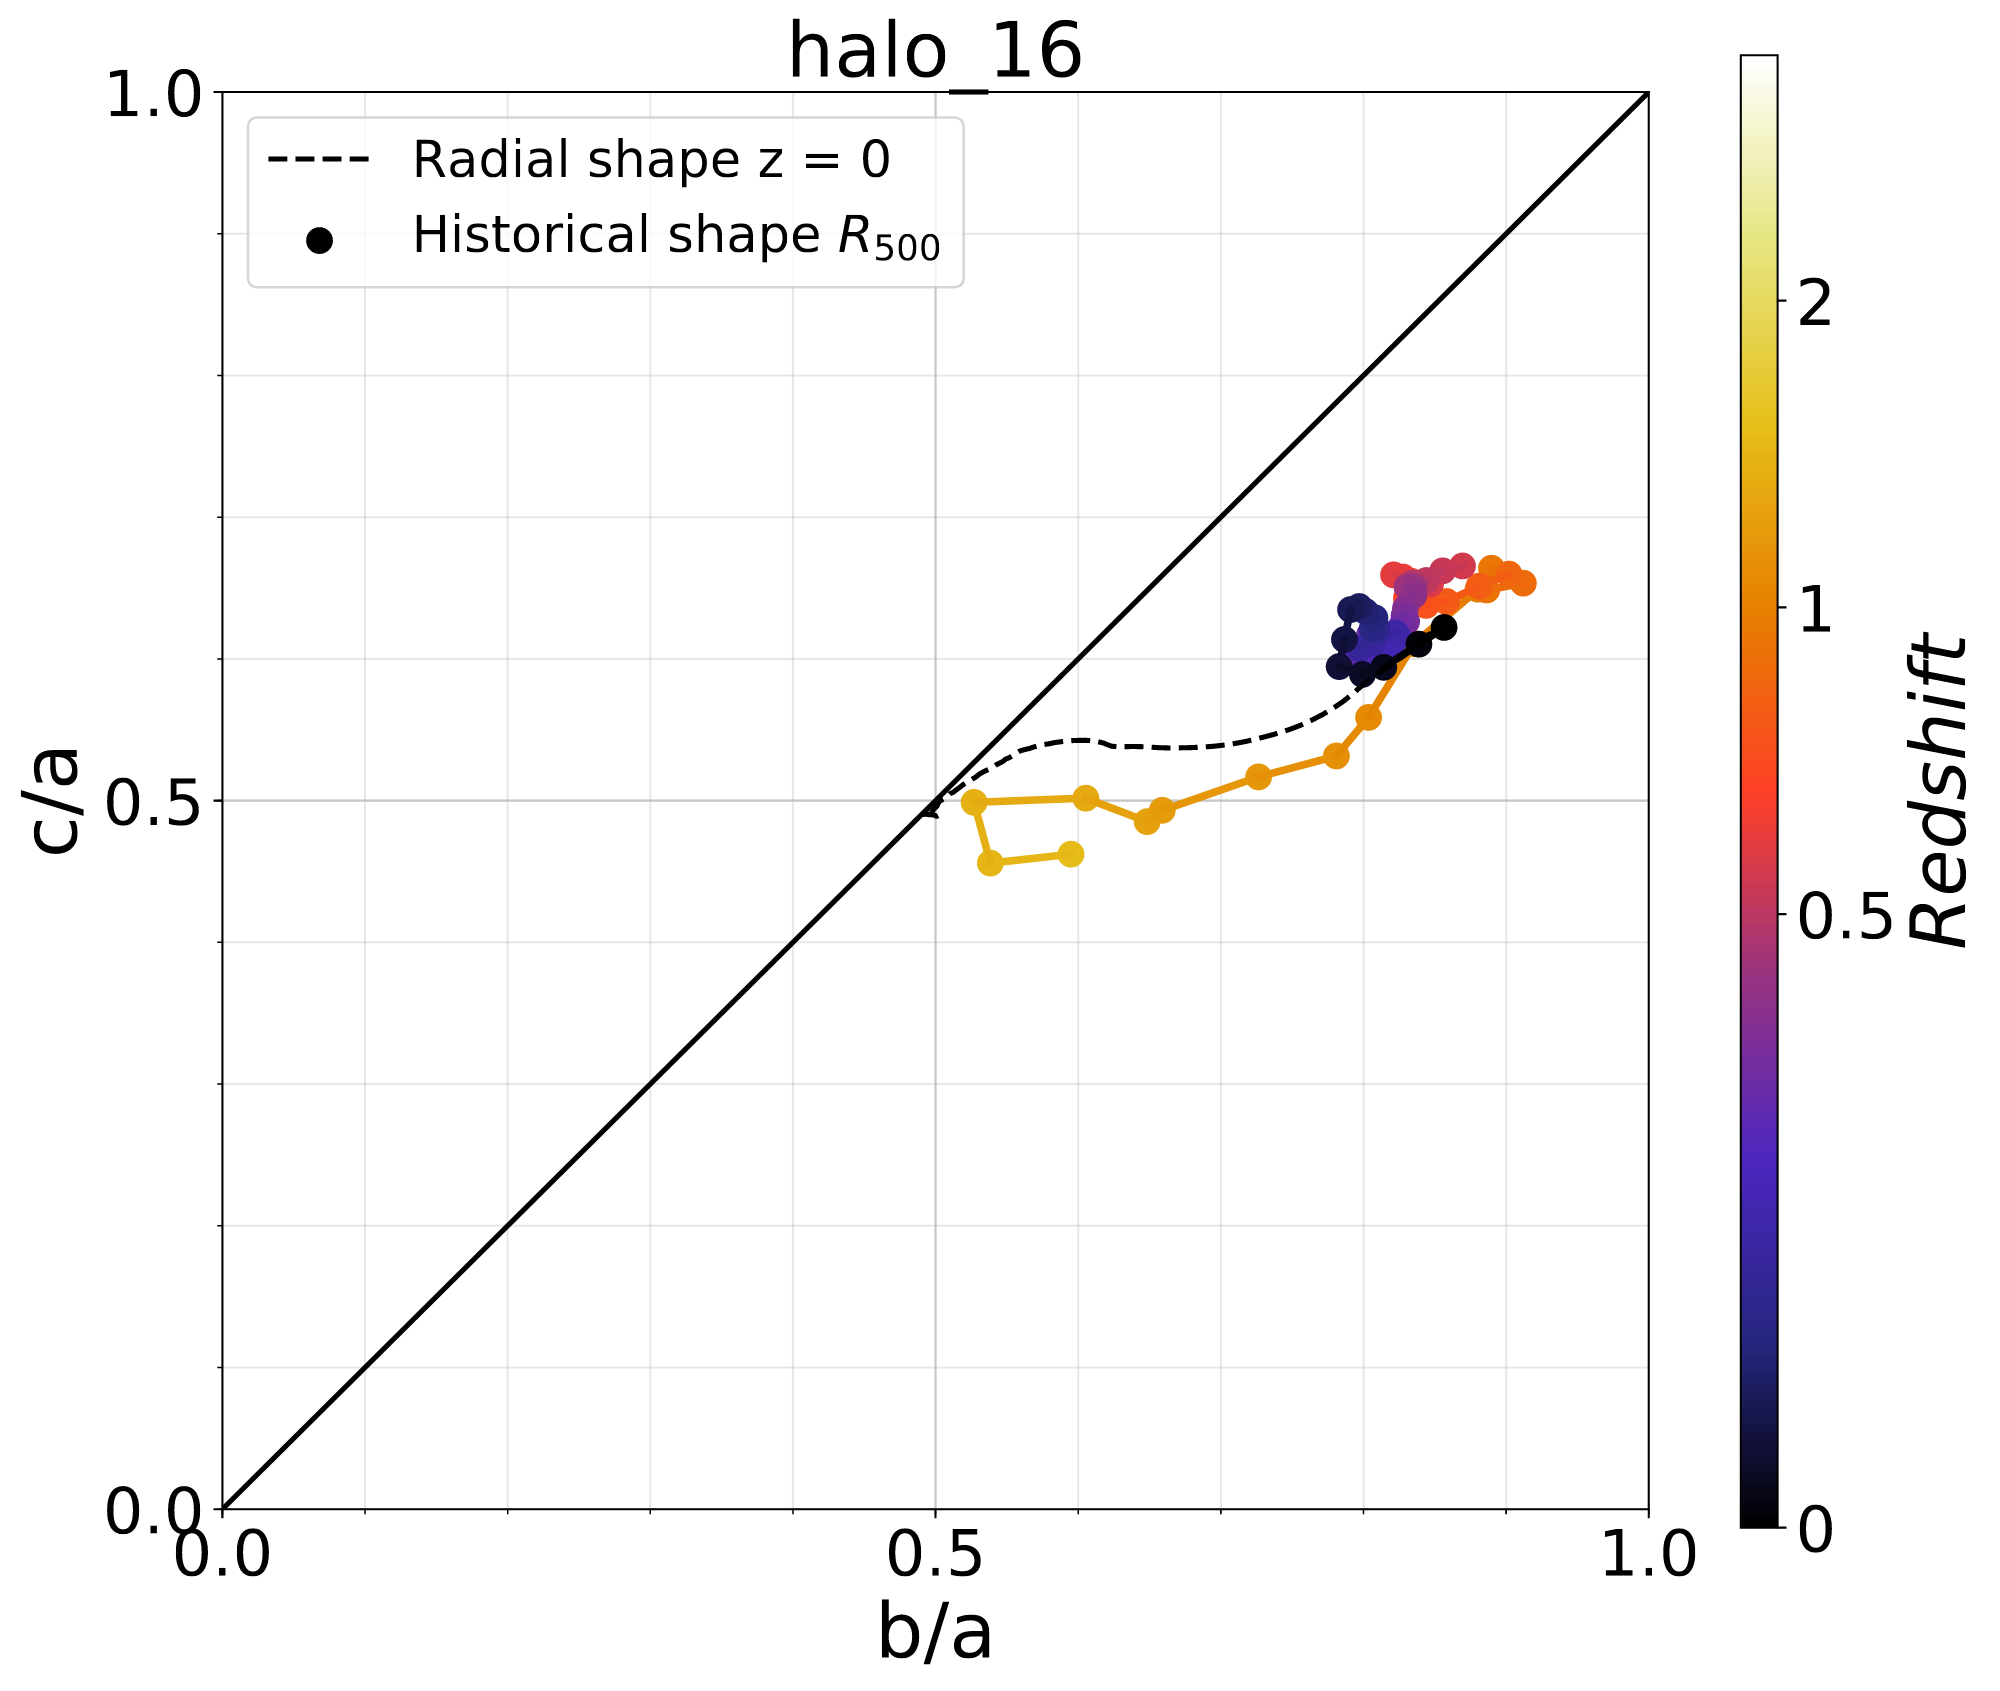
\includegraphics[width=0.5\columnwidth]{./pics/Redshift/halo_16_level3_DM_Z_Triax.png}}
  \hfill
  \subfloat[halo 21 DM]{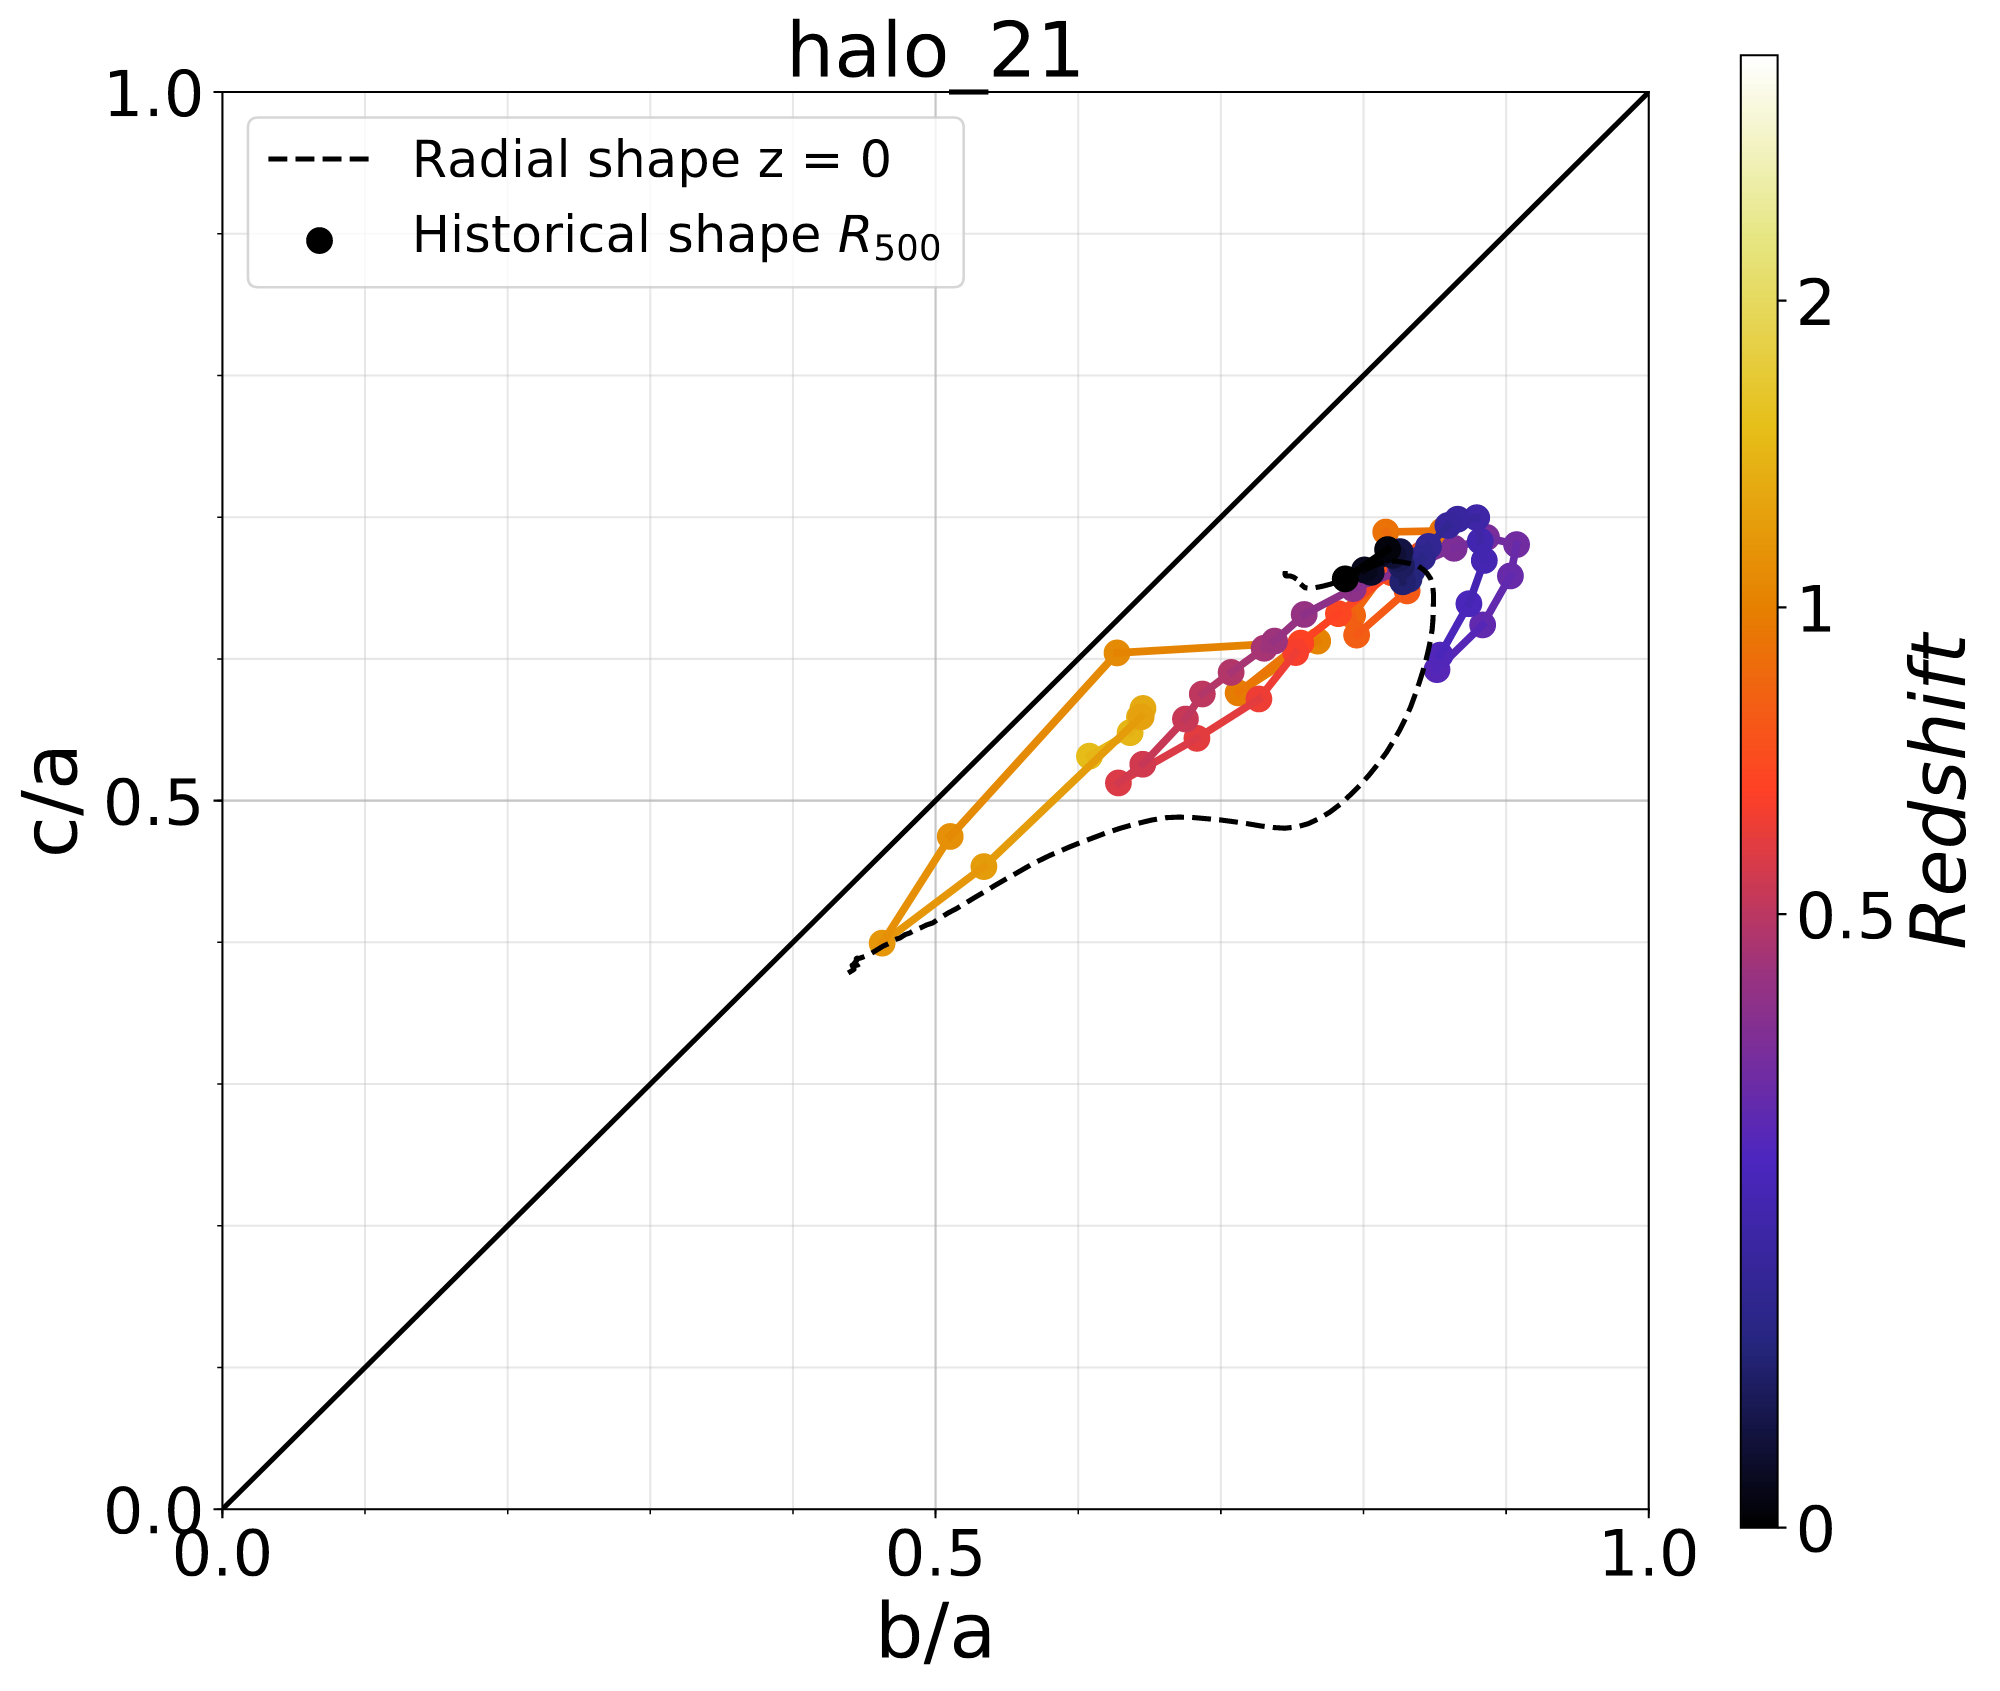
\includegraphics[width=0.5\columnwidth]{./pics/Redshift/halo_21_level3_DM_Z_Triax.png}}
  \caption{Historic shape (color dots) Vs actual radial shape (solid black line) on the Triaxiality plane. Each colored dot represents a calculated shape at R Mean 200, for each redshift. It is clear that halos with memory (halo 16), unlike disrupted halos (halo 21), have correlation between their historical and radial profiles.}
  \label{fig:RedshiftDM}
\end{figure}
%\end{verbatim}


In the case of MHD halos, we have a steady rounding effect with time but this tendency is not monotonous with radius at constant redshift, for which we deduced that this memory correlation is not evident.\\




 
